\documentclass[cn,pad,chinese,chinesefont=nofont]{elegantbook}
\usepackage{latexgit}
\usepackage{hyperref}
\usepackage{hyperxmp}
\hypersetup{
	pdftitle={Dongxiao Mannual},
    pdfauthor={xue35},
    pdfcopyright={Copyright (C) 2020 by Jianmin Xue.  All rights reserved.}
}
%\usepackage{showframe}
\setCJKmainfont{Source Han Serif} 
\setCJKsansfont{Source Han Sans} 
\setCJKmonofont{Source Han Mono} 
\setCJKfamilyfont{zhsong}{Source Han Serif}
\setCJKfamilyfont{zhhei}{Source Han Sans} 
\setCJKfamilyfont{zhkai}{Source Han Mono} 
\setCJKfamilyfont{zhfs}{Source Han Mono} 
\newcommand*{\songti}{\CJKfamily{zhsong}} 
\newcommand*{\heiti}{\CJKfamily{zhhei}} 
\newcommand*{\kaishu}{\CJKfamily{zhkai}} 
\newcommand*{\fangsong}{\CJKfamily{zhfs}}

\title{洞箫演奏入门}
\author{雪散舞}
\date{\zhtoday}
\cover{dongxiao/cover.jpeg}
\logo{monk.png}
\extrainfo{清籁远喑喑,秦楼夜思深。碧空人已去,沧海凤难寻。\\杳妙和云绝,依微向水沉。还将九成意,高阁伫芳音。}
\version{\gitcommithash}

\begin{document}
\maketitle
\frontmatter
\tableofcontents
\mainmatter

\centering
\chapter{筒音做‘低音2’}
\section{指法表}
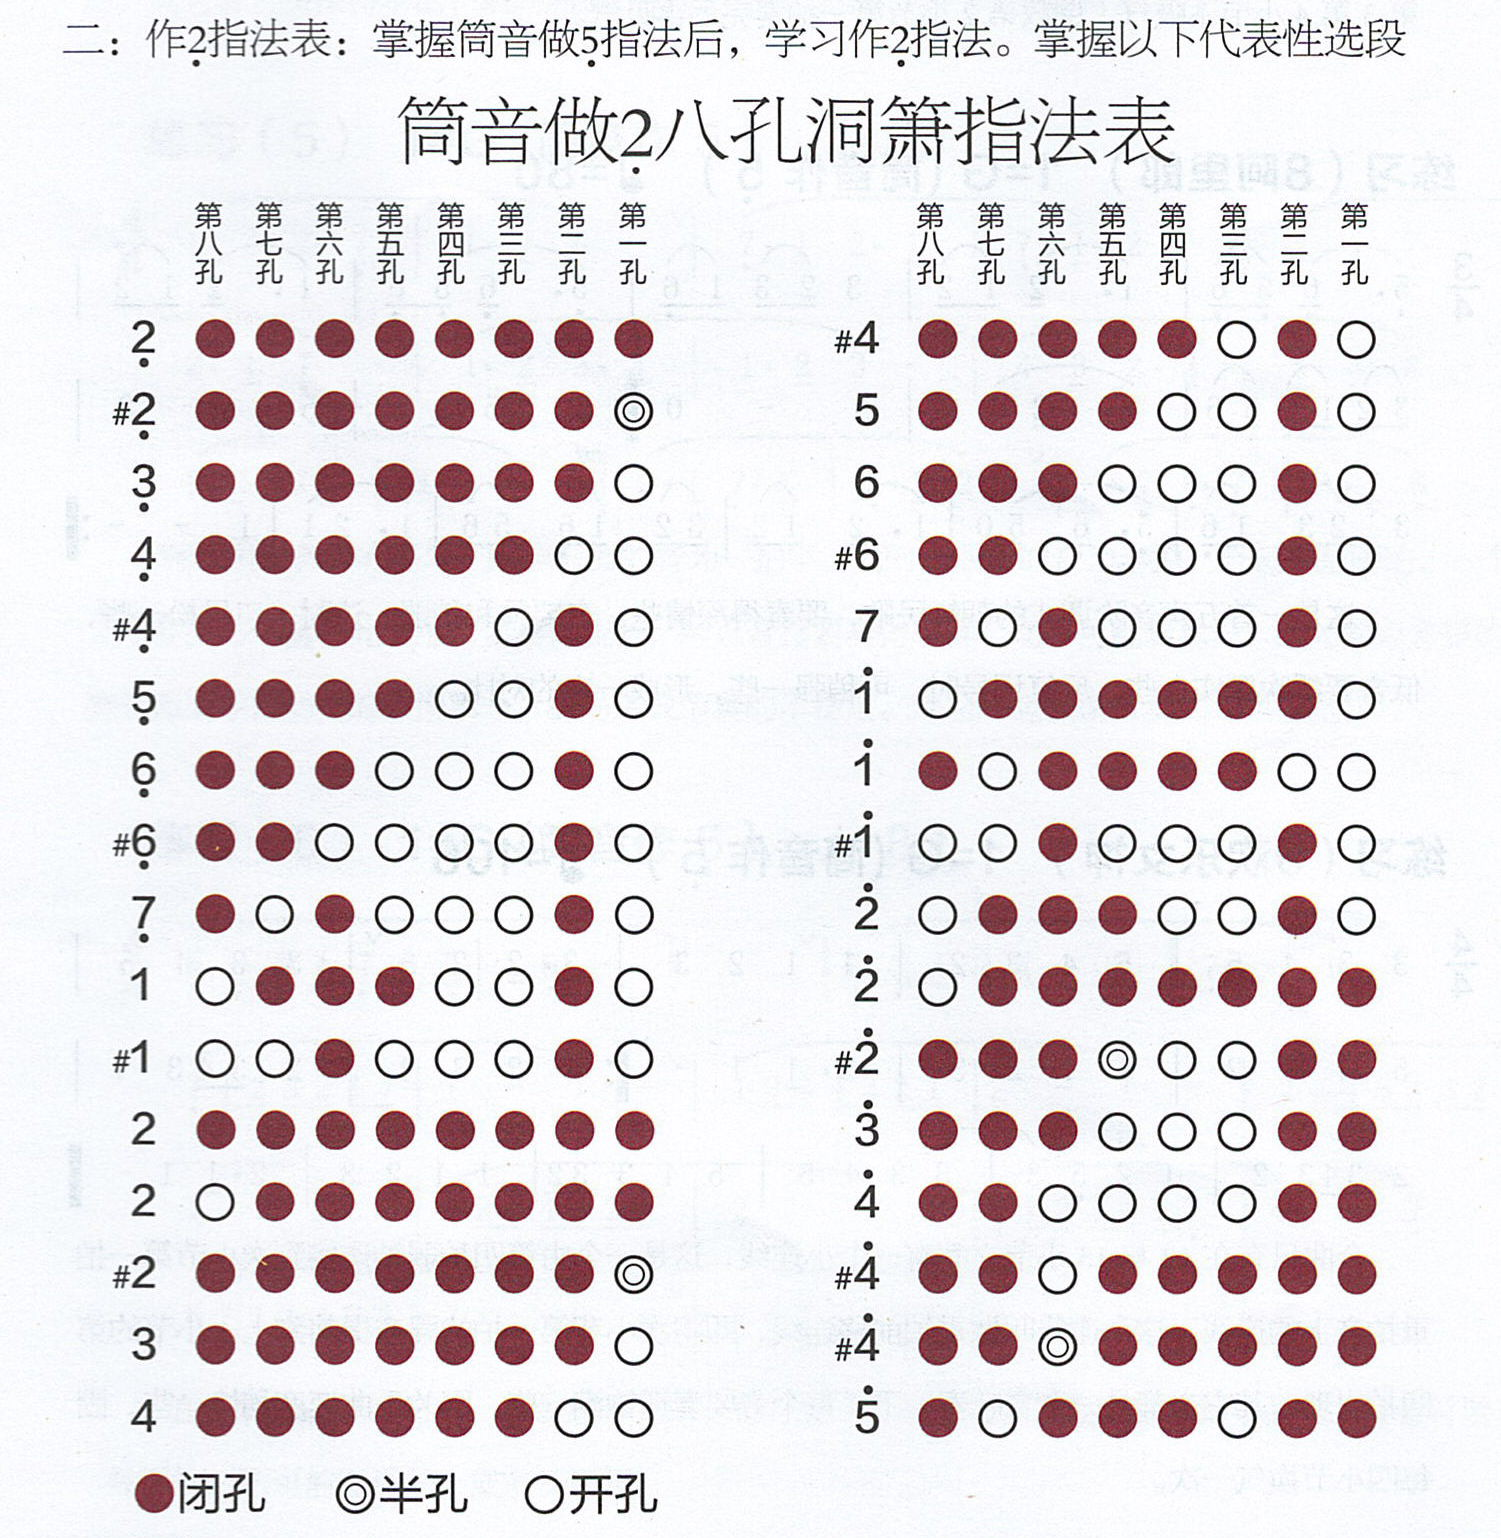
\includegraphics[width=\textwidth]{dongxiao/Scan 4.1.jpeg}

\section{练习(1-2)C调}
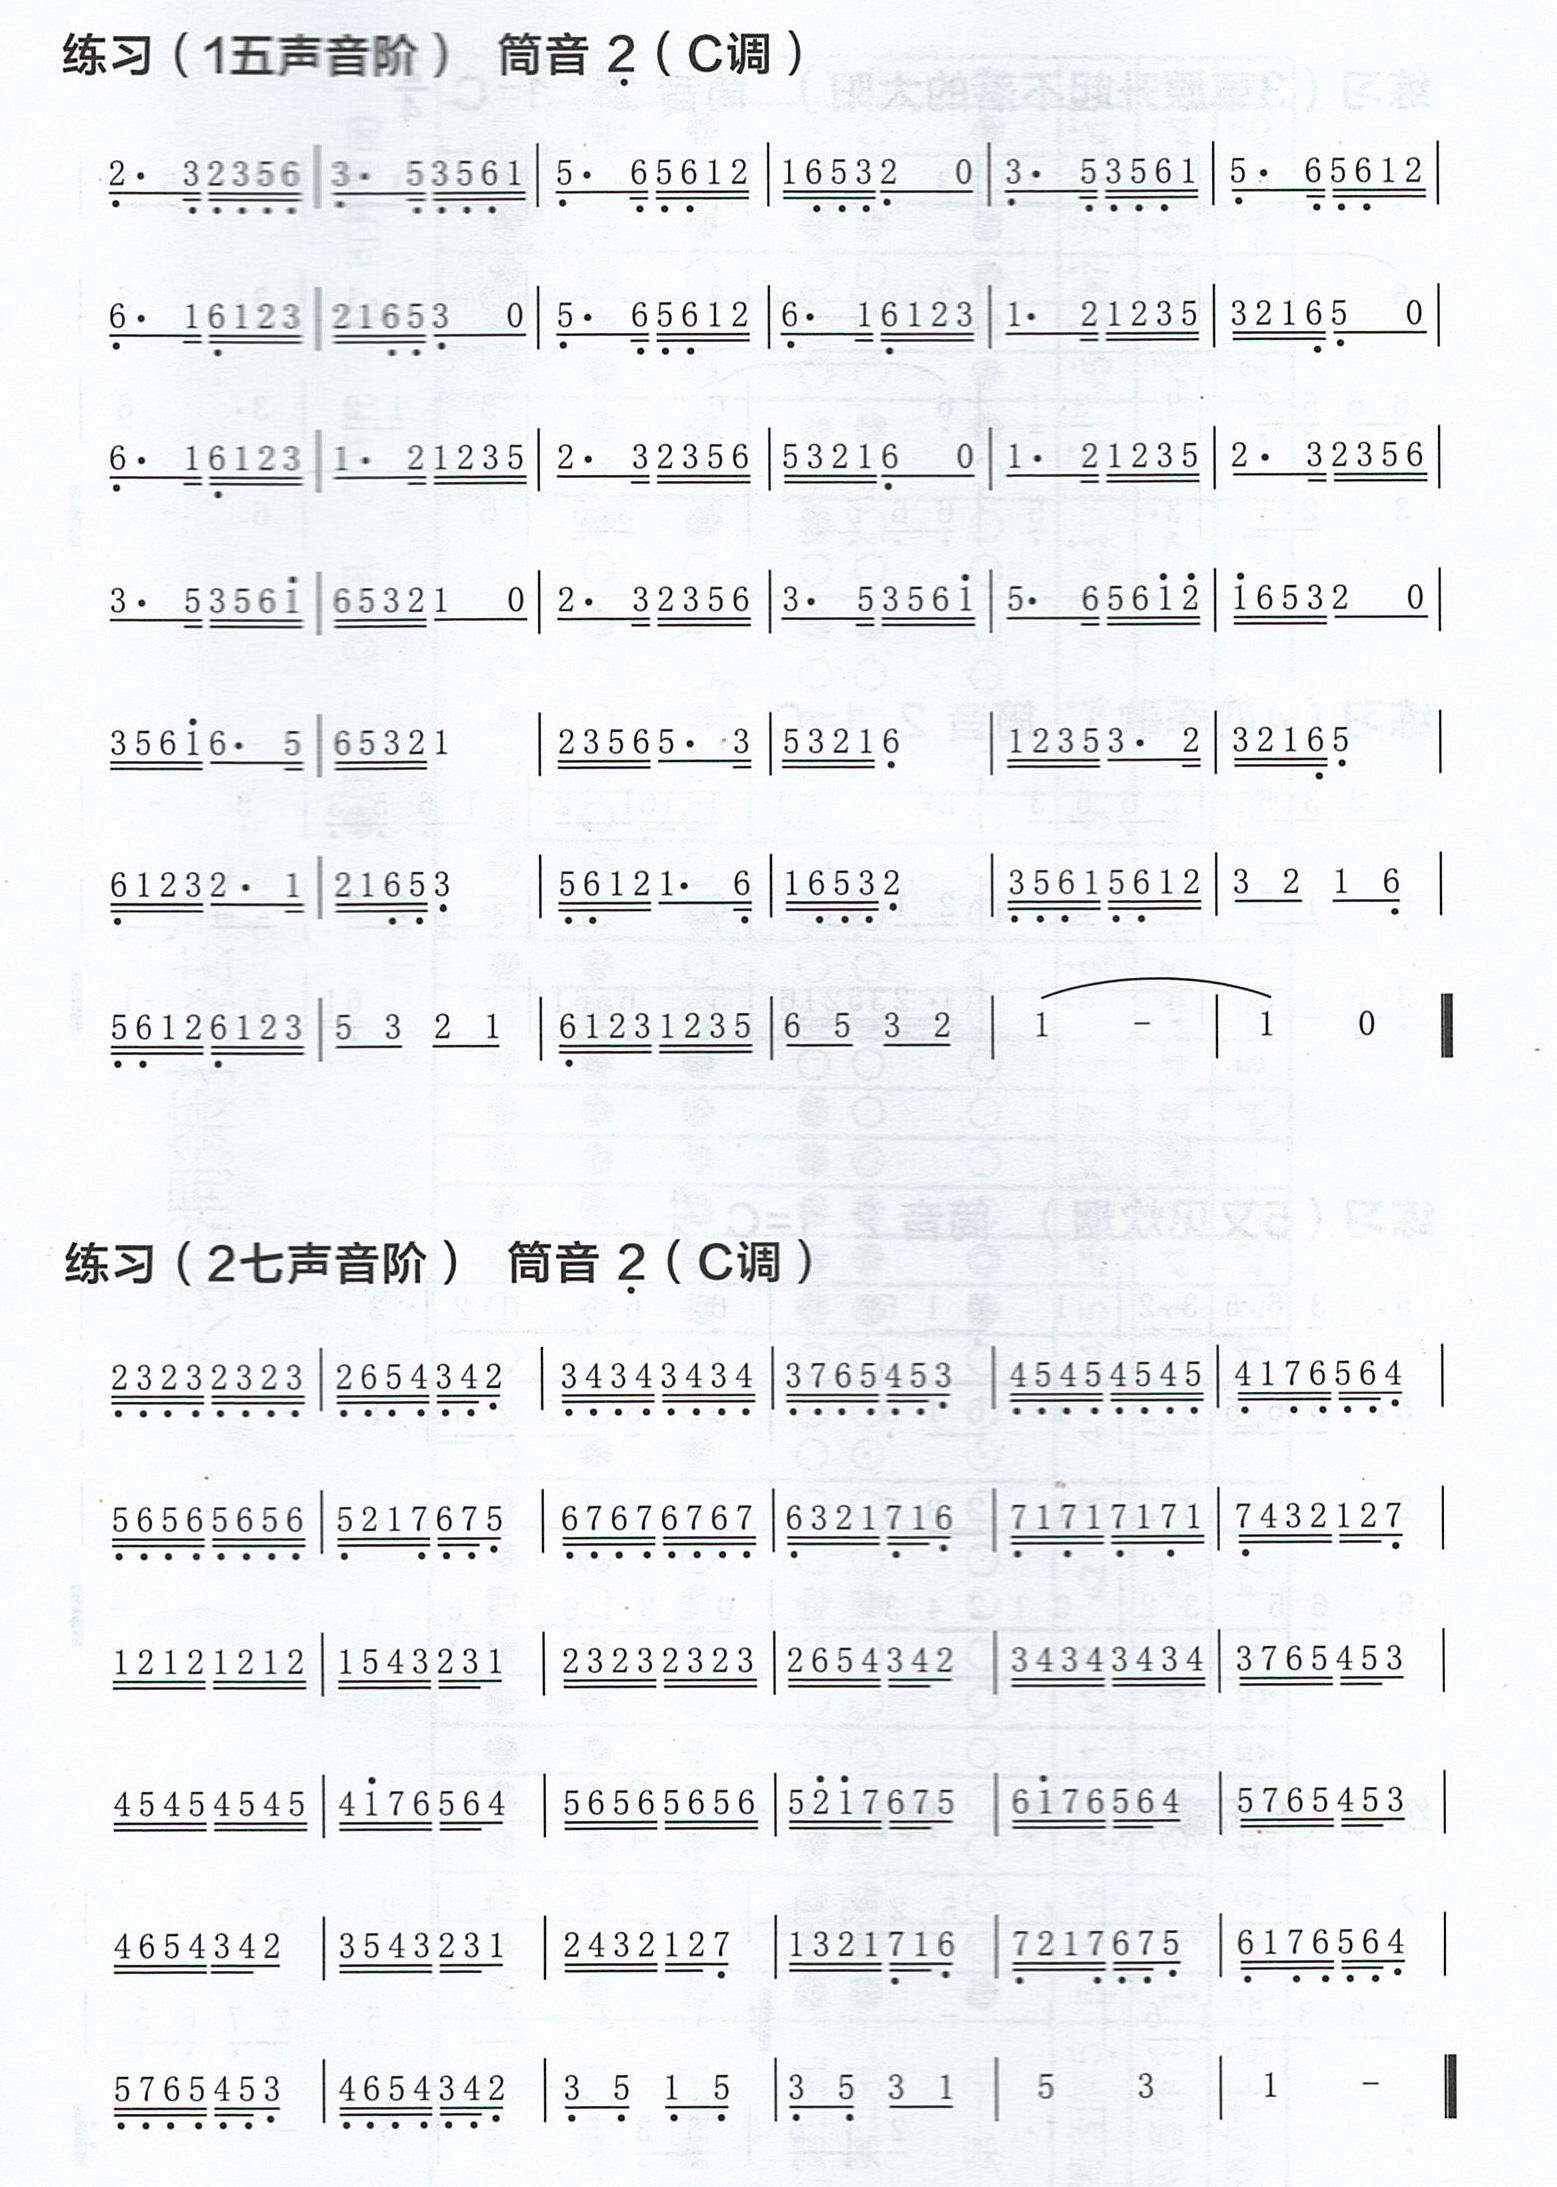
\includegraphics[height=\textheight]{dongxiao/Scan 5.jpeg}

\section{练习(3草原上升起不落的太阳2/4,4四季歌2/4 5又见炊烟4/4 6沂蒙山小调3/4)1=C}
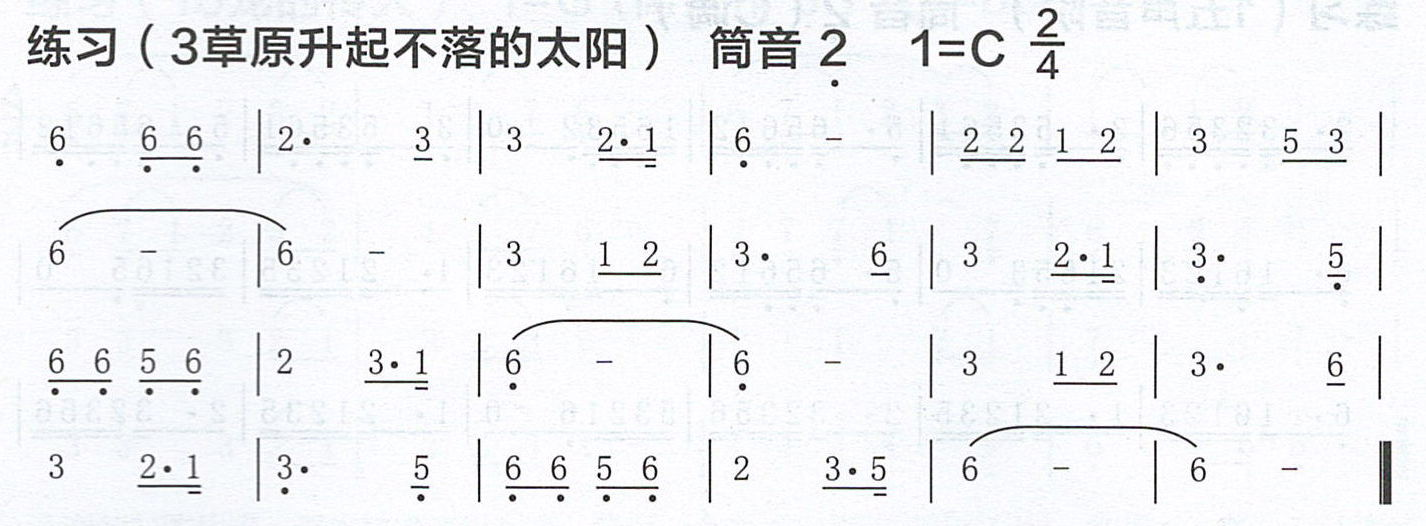
\includegraphics[height=0.9\textheight]{dongxiao/Scan 6.jpeg}

\chapter{筒音做‘低音2’-曲谱练习}

\section{卖报歌}
	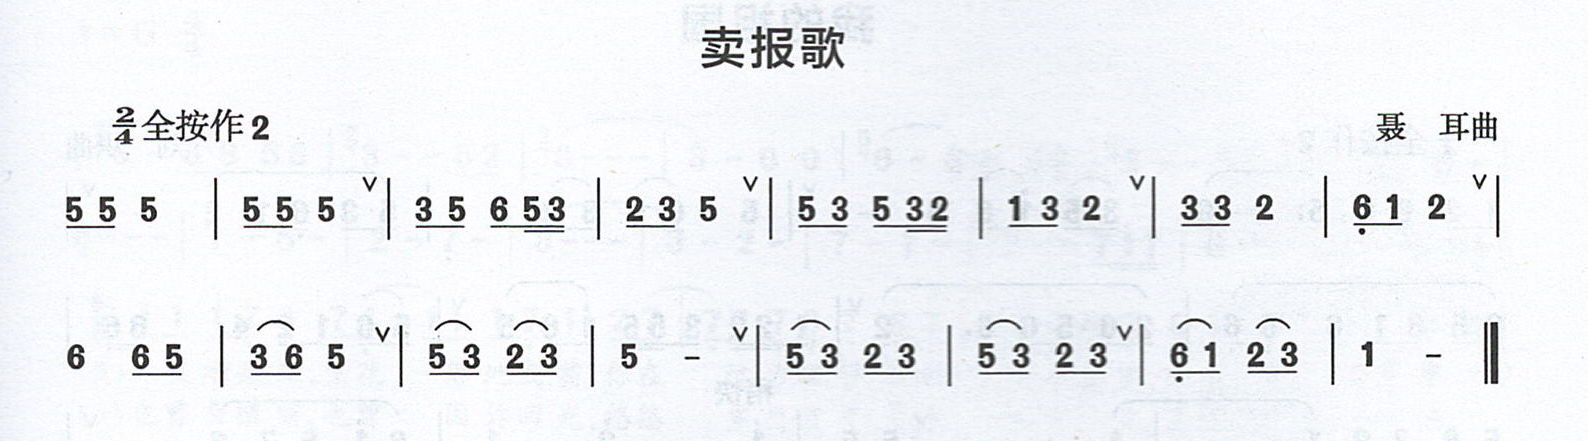
\includegraphics[width=\textwidth]{dongxiao/Scan 18-1.jpeg}
\section{沂蒙山小调}
	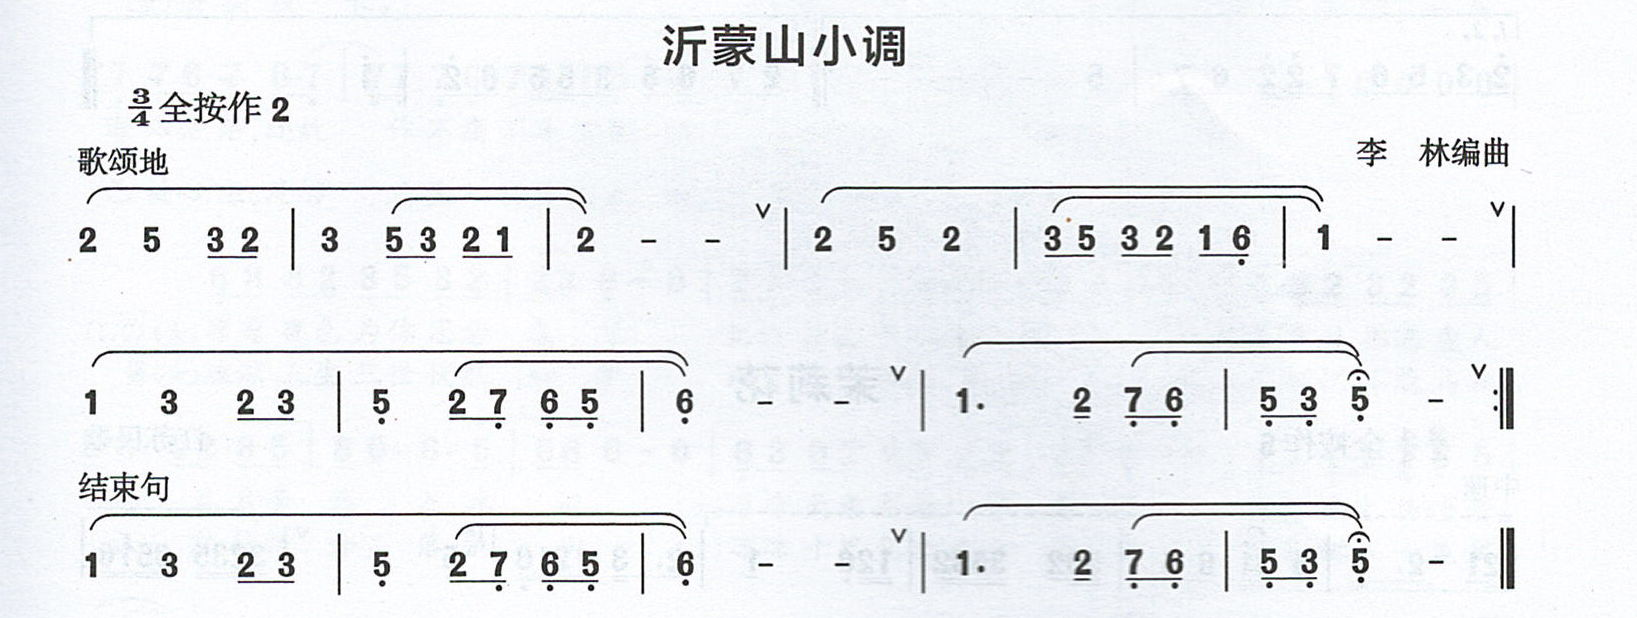
\includegraphics[width=\textwidth]{dongxiao/Scan 18-2.jpeg}
\section{康定情歌}
	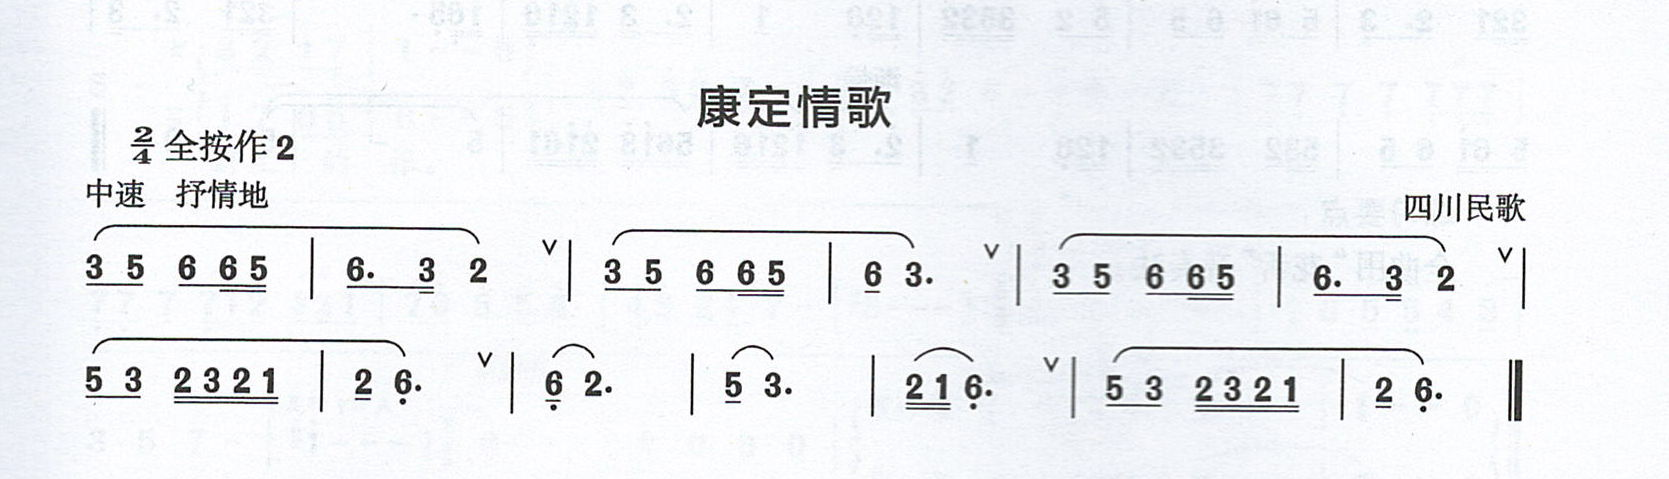
\includegraphics[width=\textwidth]{dongxiao/Scan 18-3.jpeg}

\section{我的祖国}
	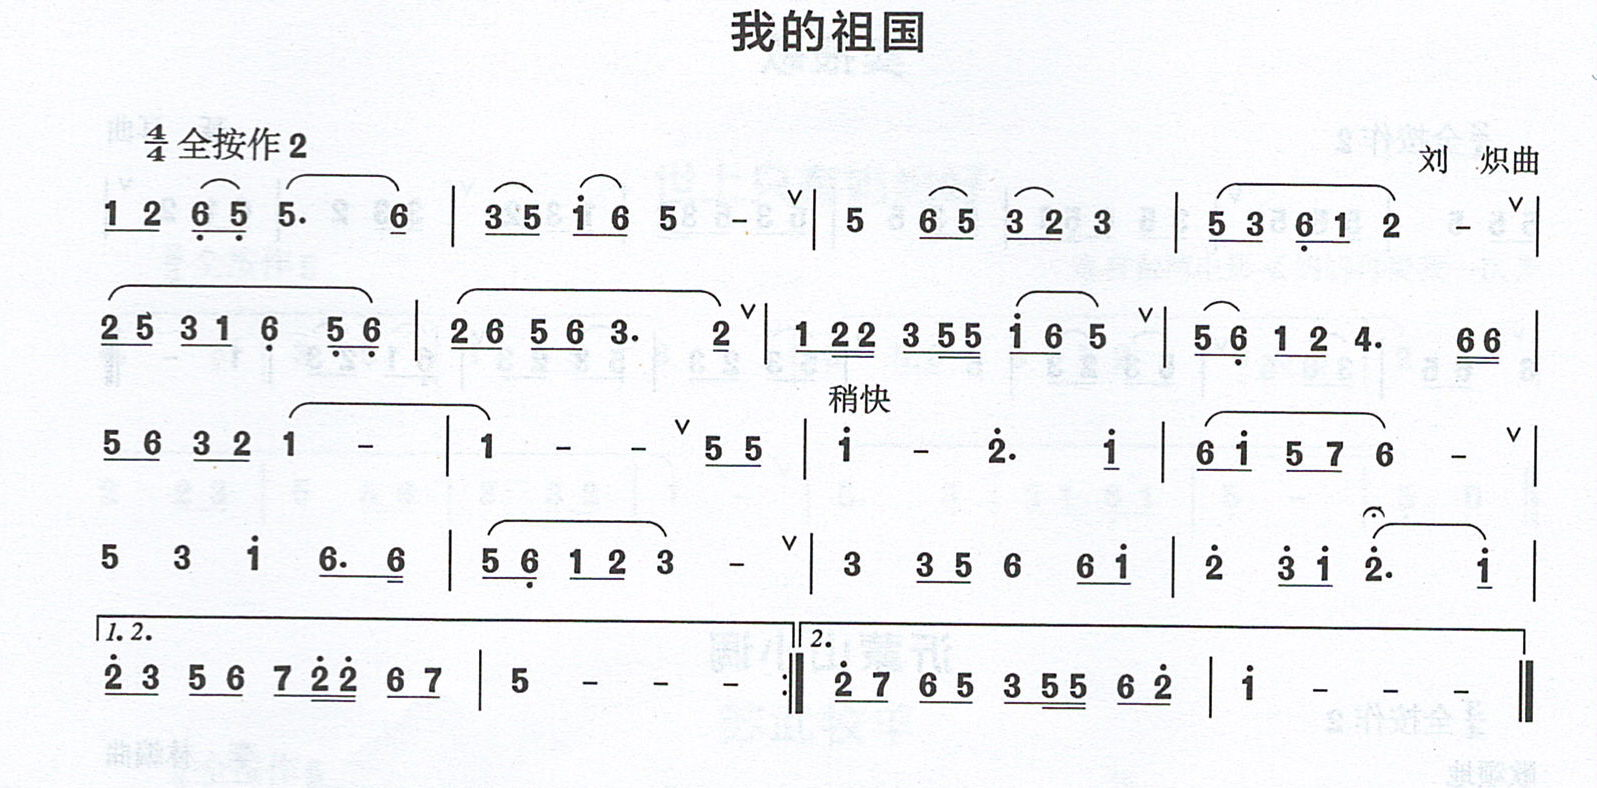
\includegraphics[width=\textwidth]{dongxiao/Scan 19-1.jpeg}

\section{小草}
	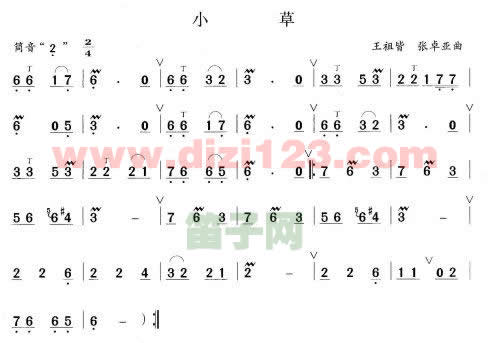
\includegraphics[width=\textwidth]{dongxiao/小草.jpg}
\section{一样的人}
	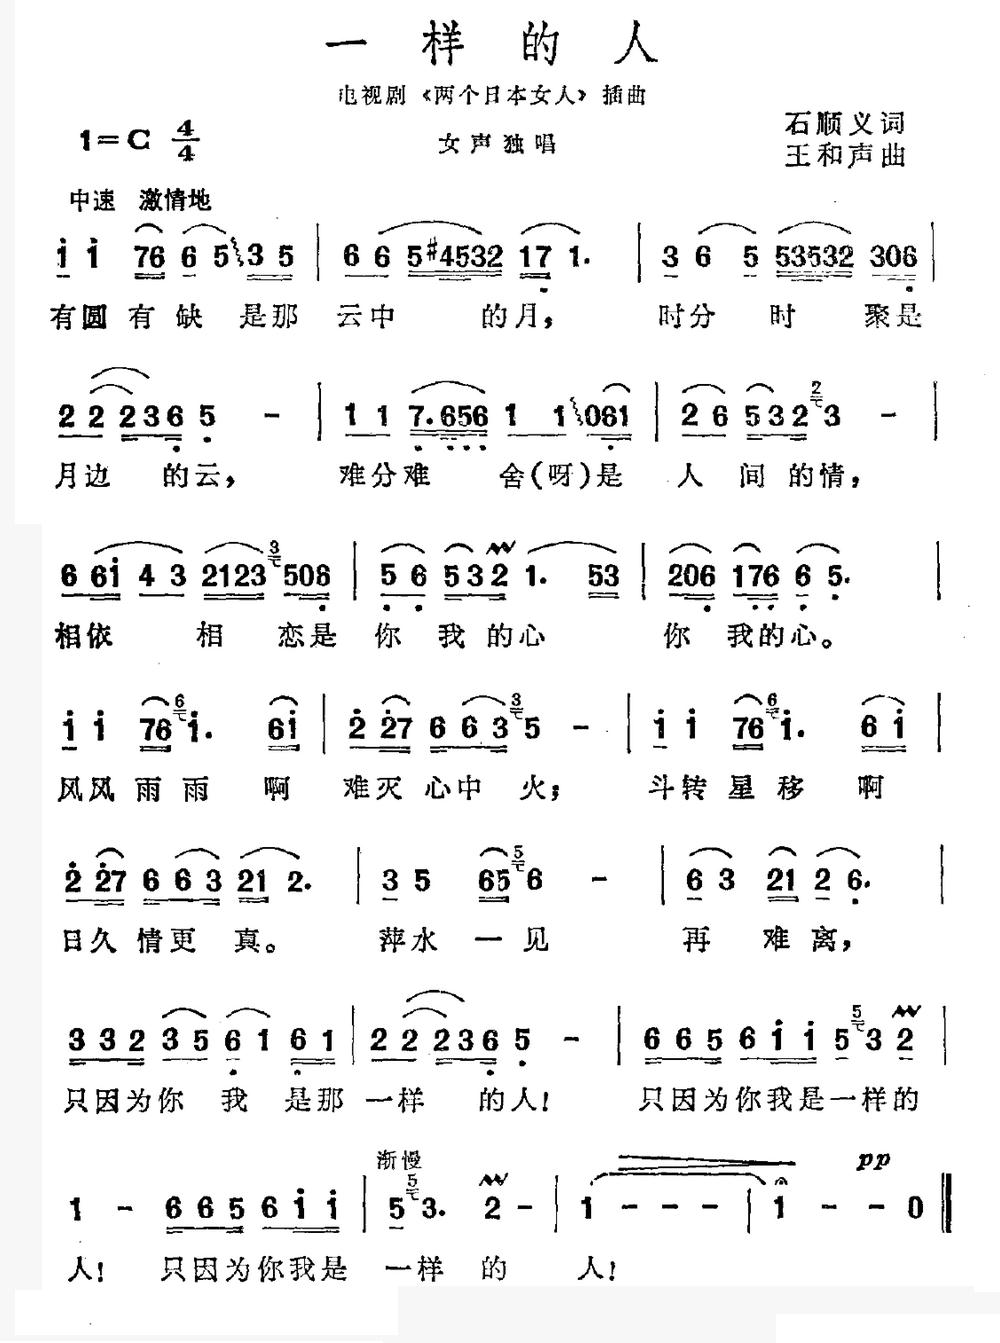
\includegraphics[height=\textheight]{dongxiao/日本-一样的人.jpg}
\section{八木调}
	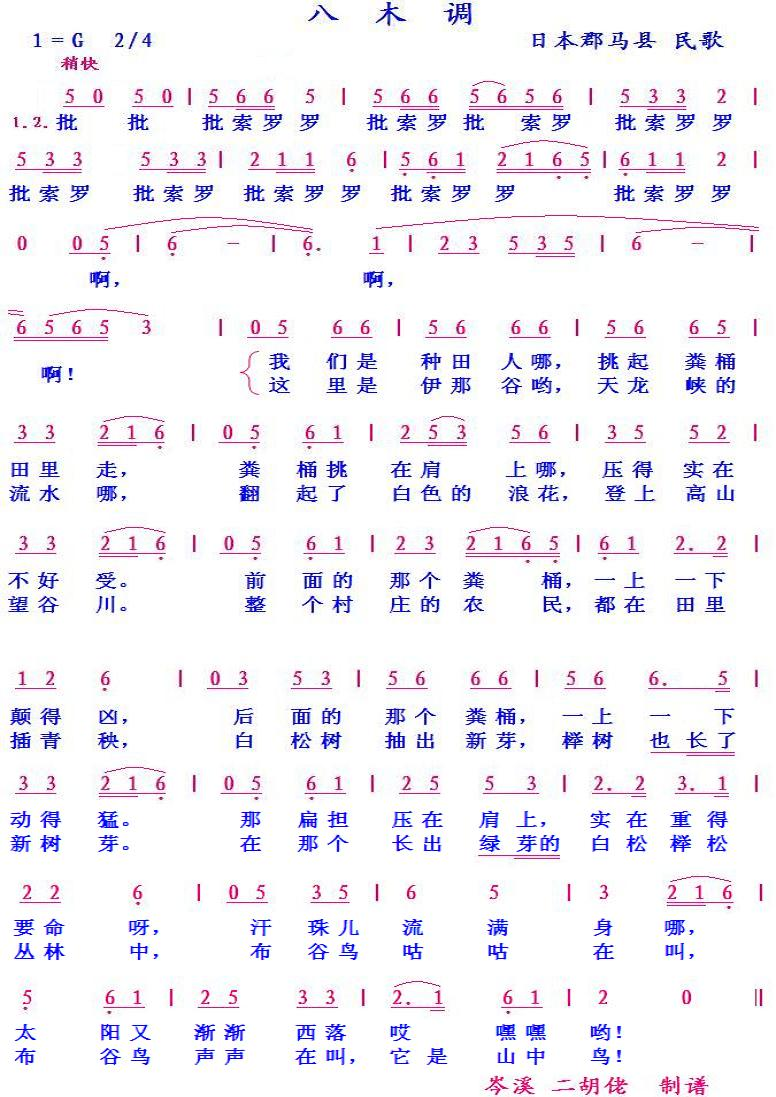
\includegraphics[height=0.9\textheight]{dongxiao/日本-八木调.jpg}
\section{去野游}
	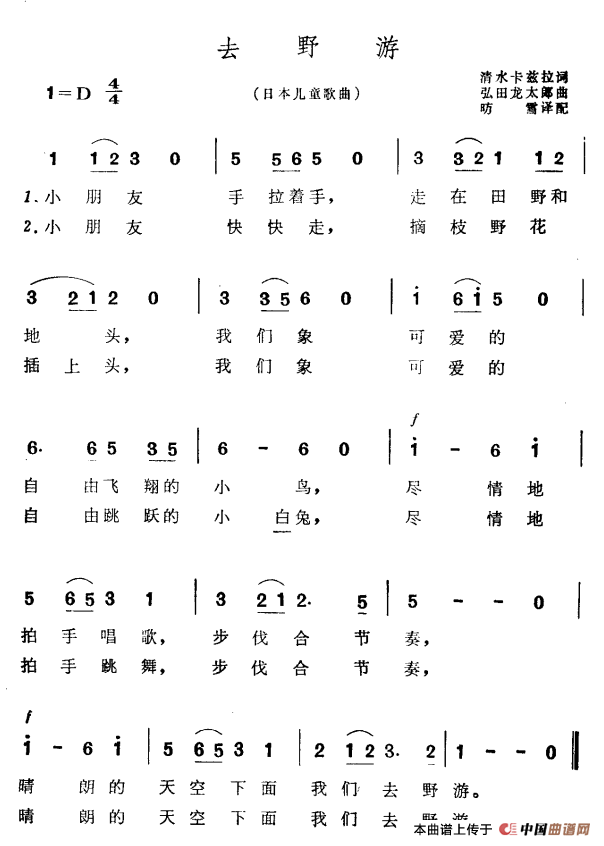
\includegraphics[height=0.9\textheight]{dongxiao/日本-去野游.png}

\section{小路}
	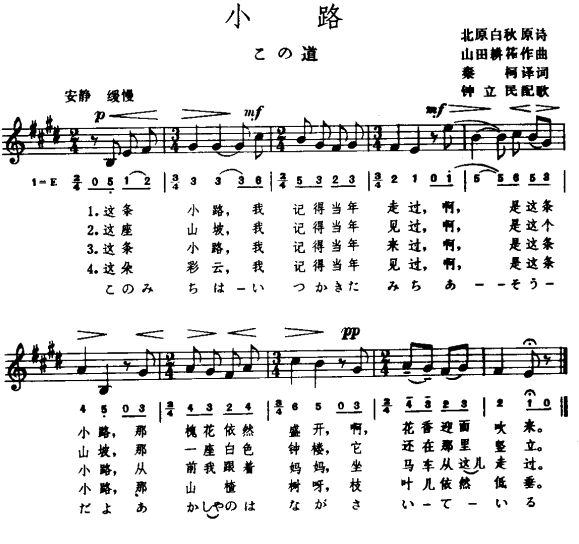
\includegraphics[width=\textwidth]{dongxiao/日本-小路.png}
\section{故乡}
	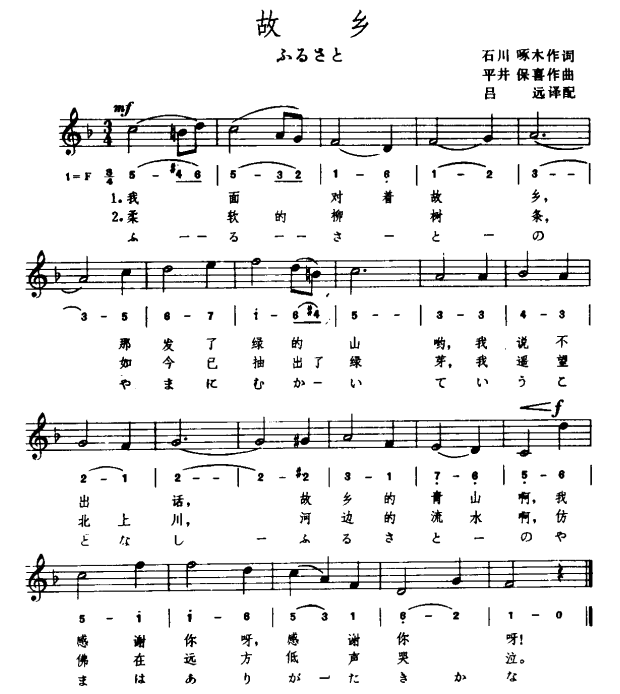
\includegraphics[width=\textwidth]{dongxiao/日本-故乡.png}
\section{春之歌}
    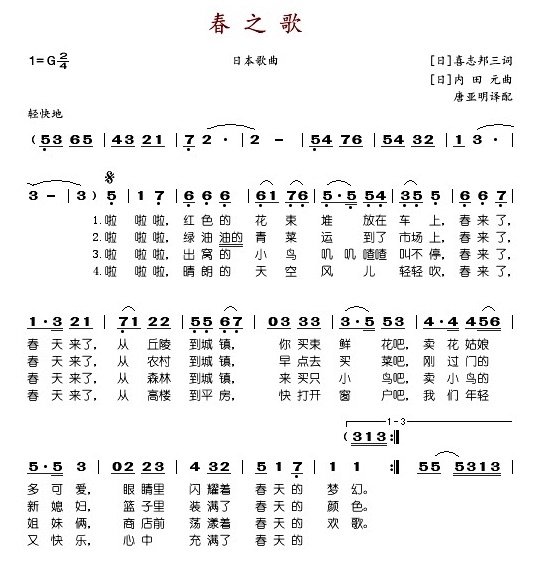
\includegraphics[width=\textwidth]{dongxiao/日本-春之歌.jpg}
\section{樱花}
	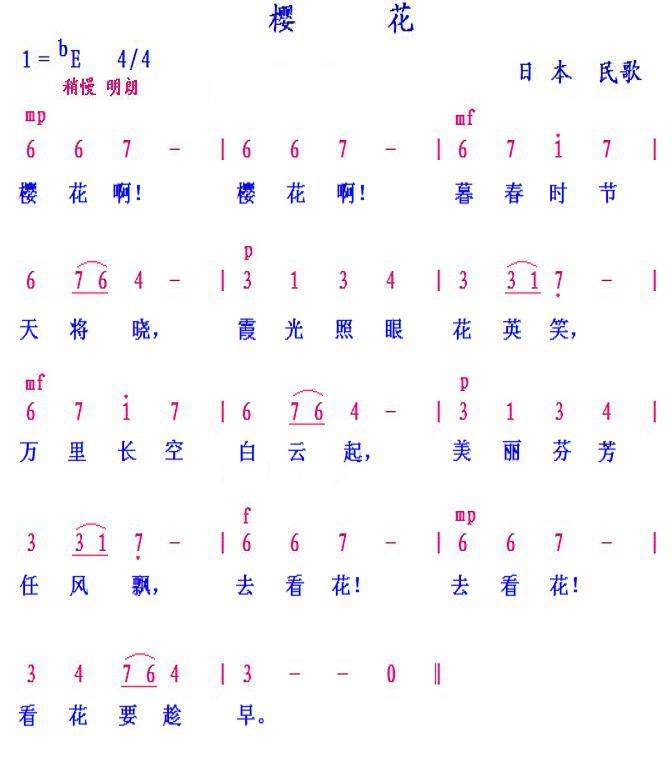
\includegraphics[width=\textwidth]{dongxiao/日本-樱花.jpg}
\section{母亲}
	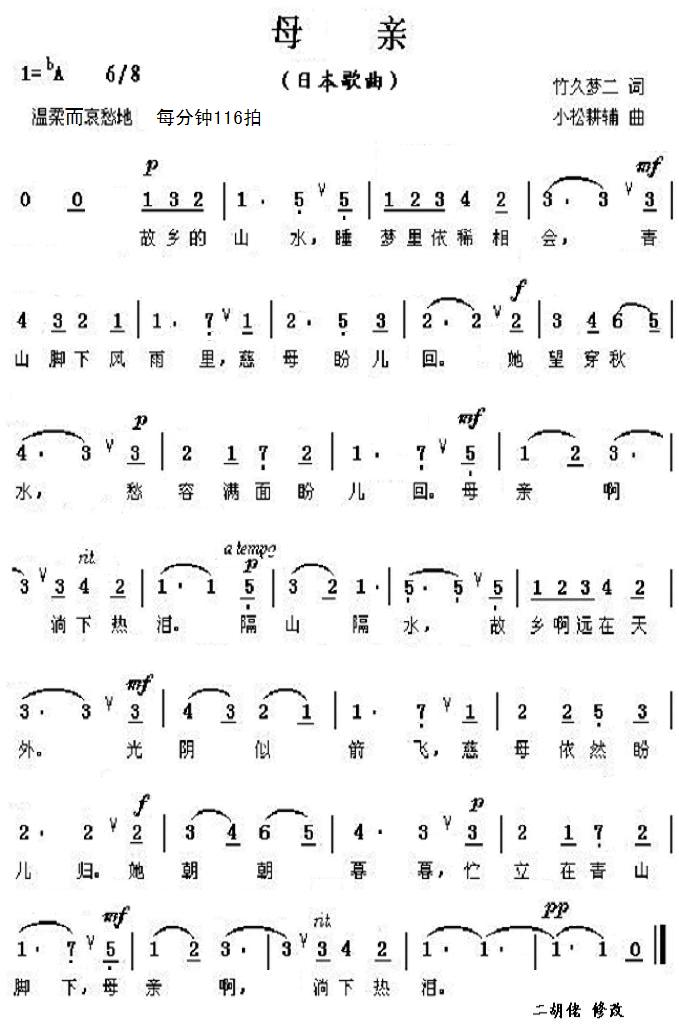
\includegraphics[height=0.9\textheight]{dongxiao/日本-母亲.jpg}

\section{洁白的雪花}
    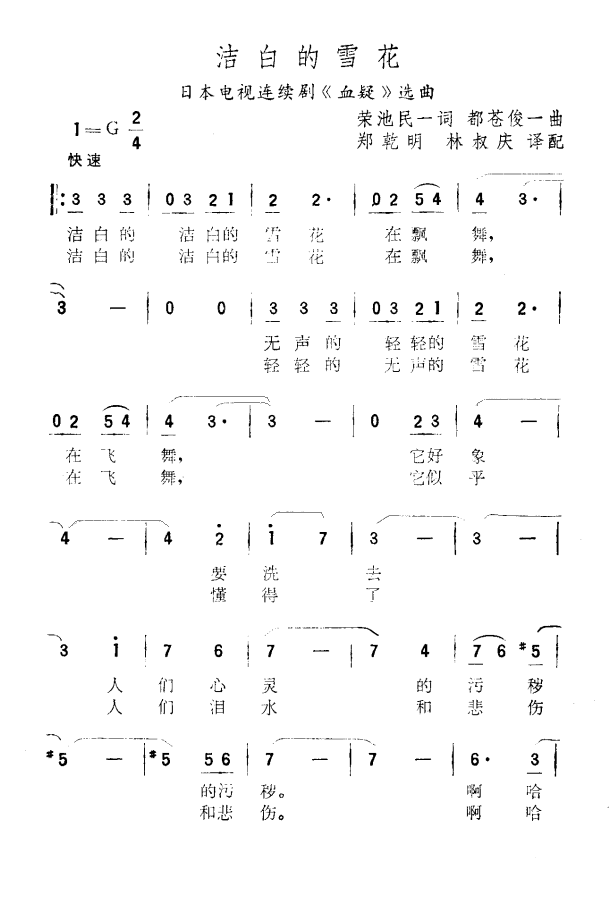
\includegraphics[height=0.9\textheight]{dongxiao/日本-洁白的雪花.png}
\section{海边之歌}
    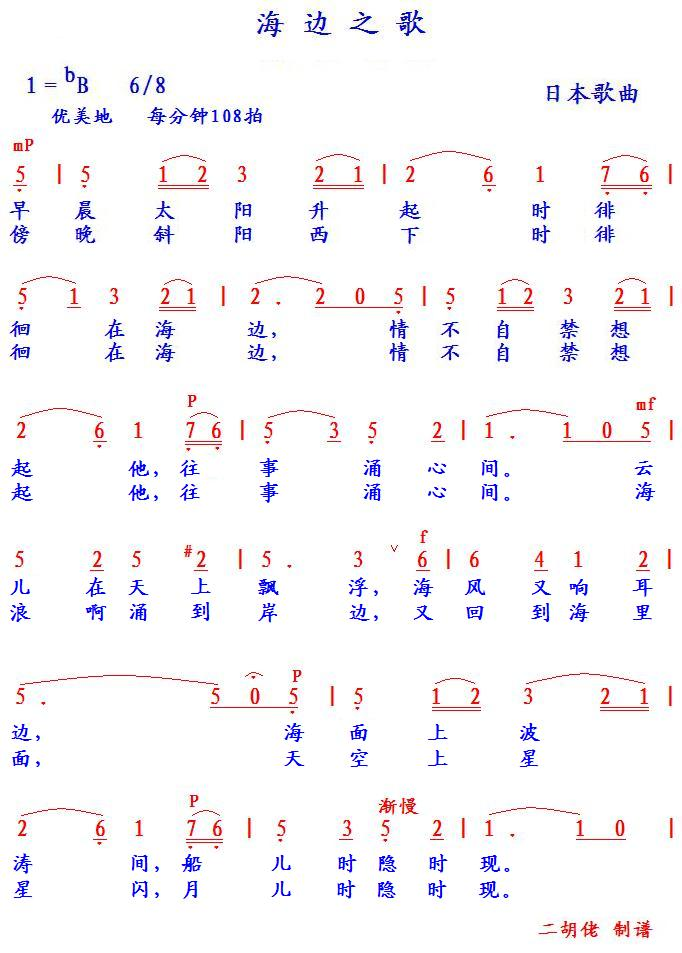
\includegraphics[height=\textheight]{dongxiao/日本-海边之歌.jpg}
\section{白云姑娘}
    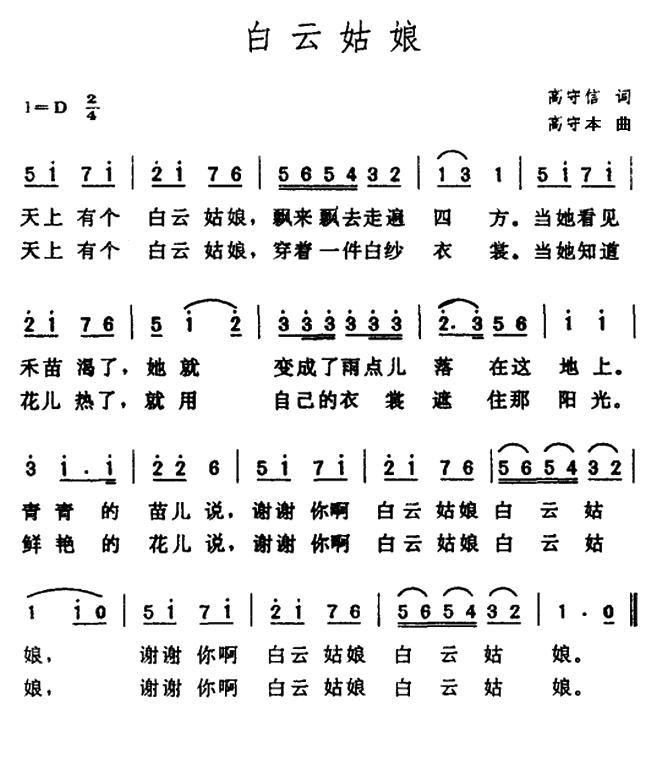
\includegraphics[width=\textwidth]{dongxiao/日本-白云姑娘.jpg}
\section{雨中岚山}
    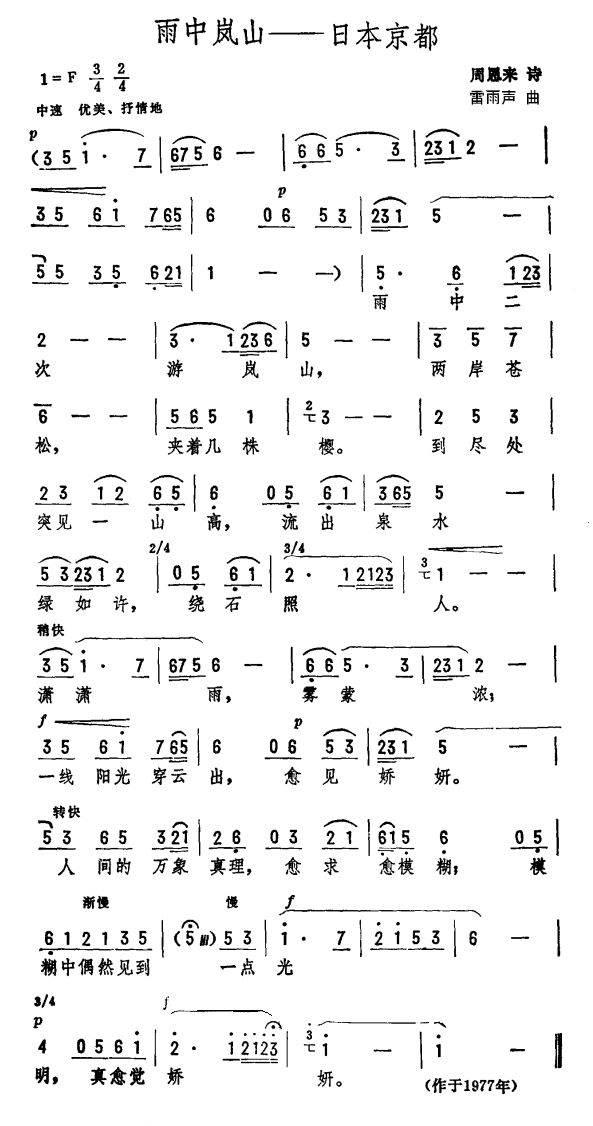
\includegraphics[height=\textheight]{dongxiao/日本-雨中岚山.png}
\section{鹰}
    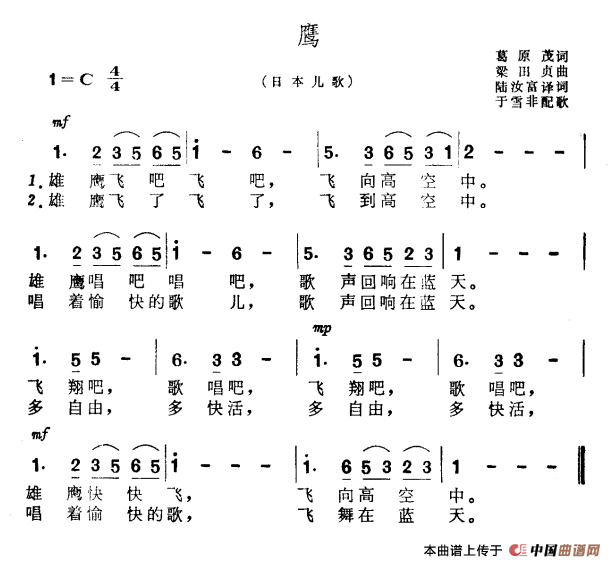
\includegraphics[width=\textwidth]{dongxiao/日本-鹰.png}

\section{洞箫悠悠}
    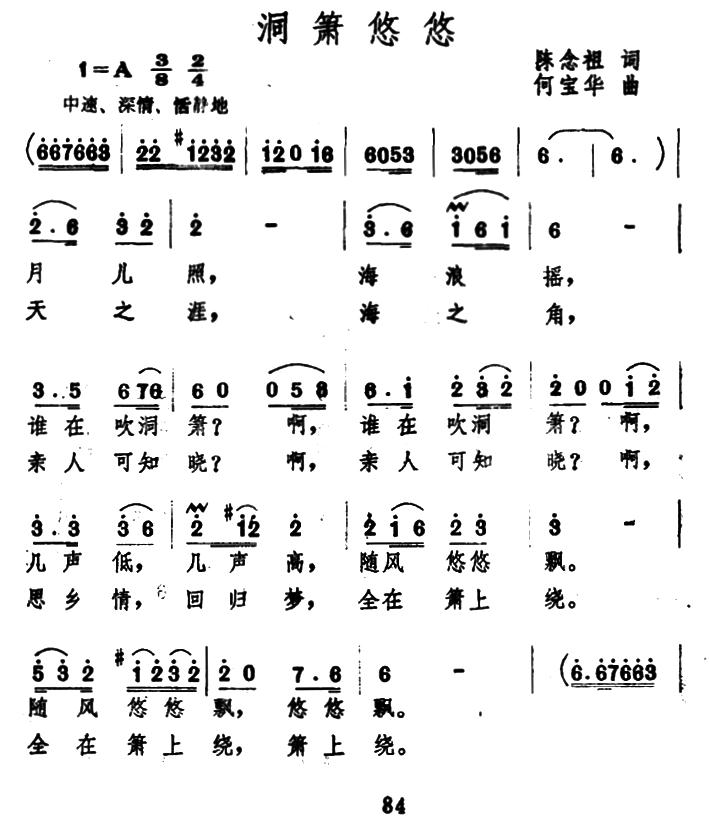
\includegraphics[width=\textwidth]{dongxiao/洞箫悠悠.jpg}
\section{红楼梦引}
    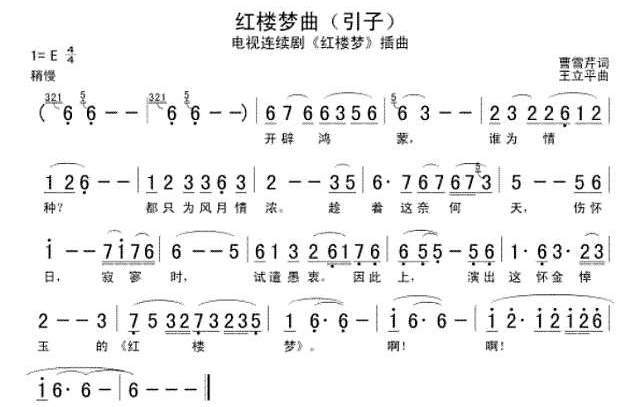
\includegraphics[width=\textwidth]{dongxiao/红楼梦引.jpg}
\section{西湖春}
    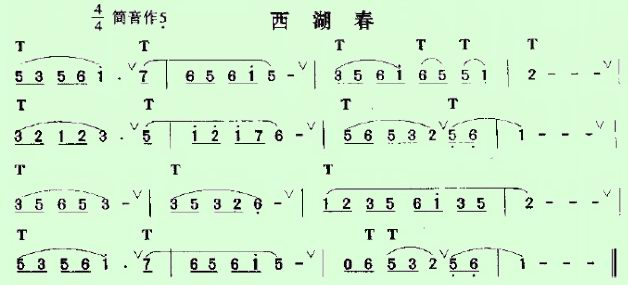
\includegraphics[width=\textwidth]{dongxiao/西湖春.jpg}

    
\section{月夜思念}
    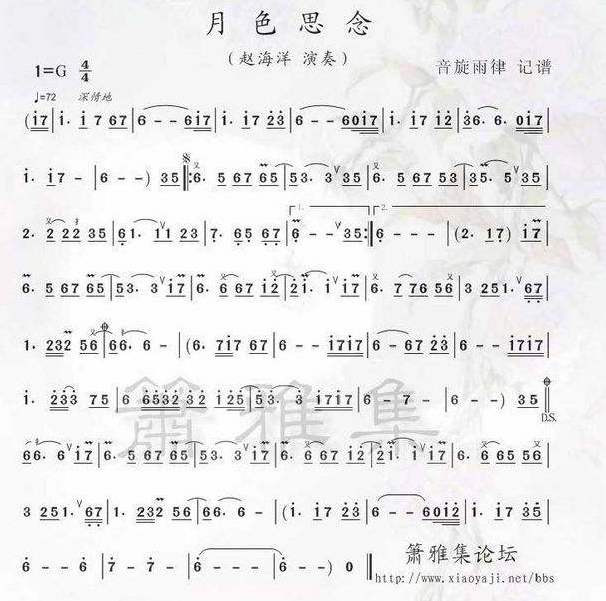
\includegraphics[width=\textwidth]{dongxiao/月夜思念.jpg}
\section{铁血丹心}
    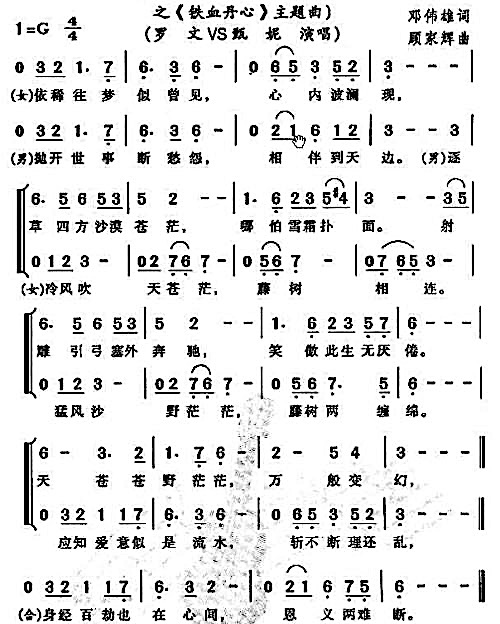
\includegraphics[width=\textwidth]{dongxiao/铁血丹心.jpg}
    
\section{青玉按-元夕}
    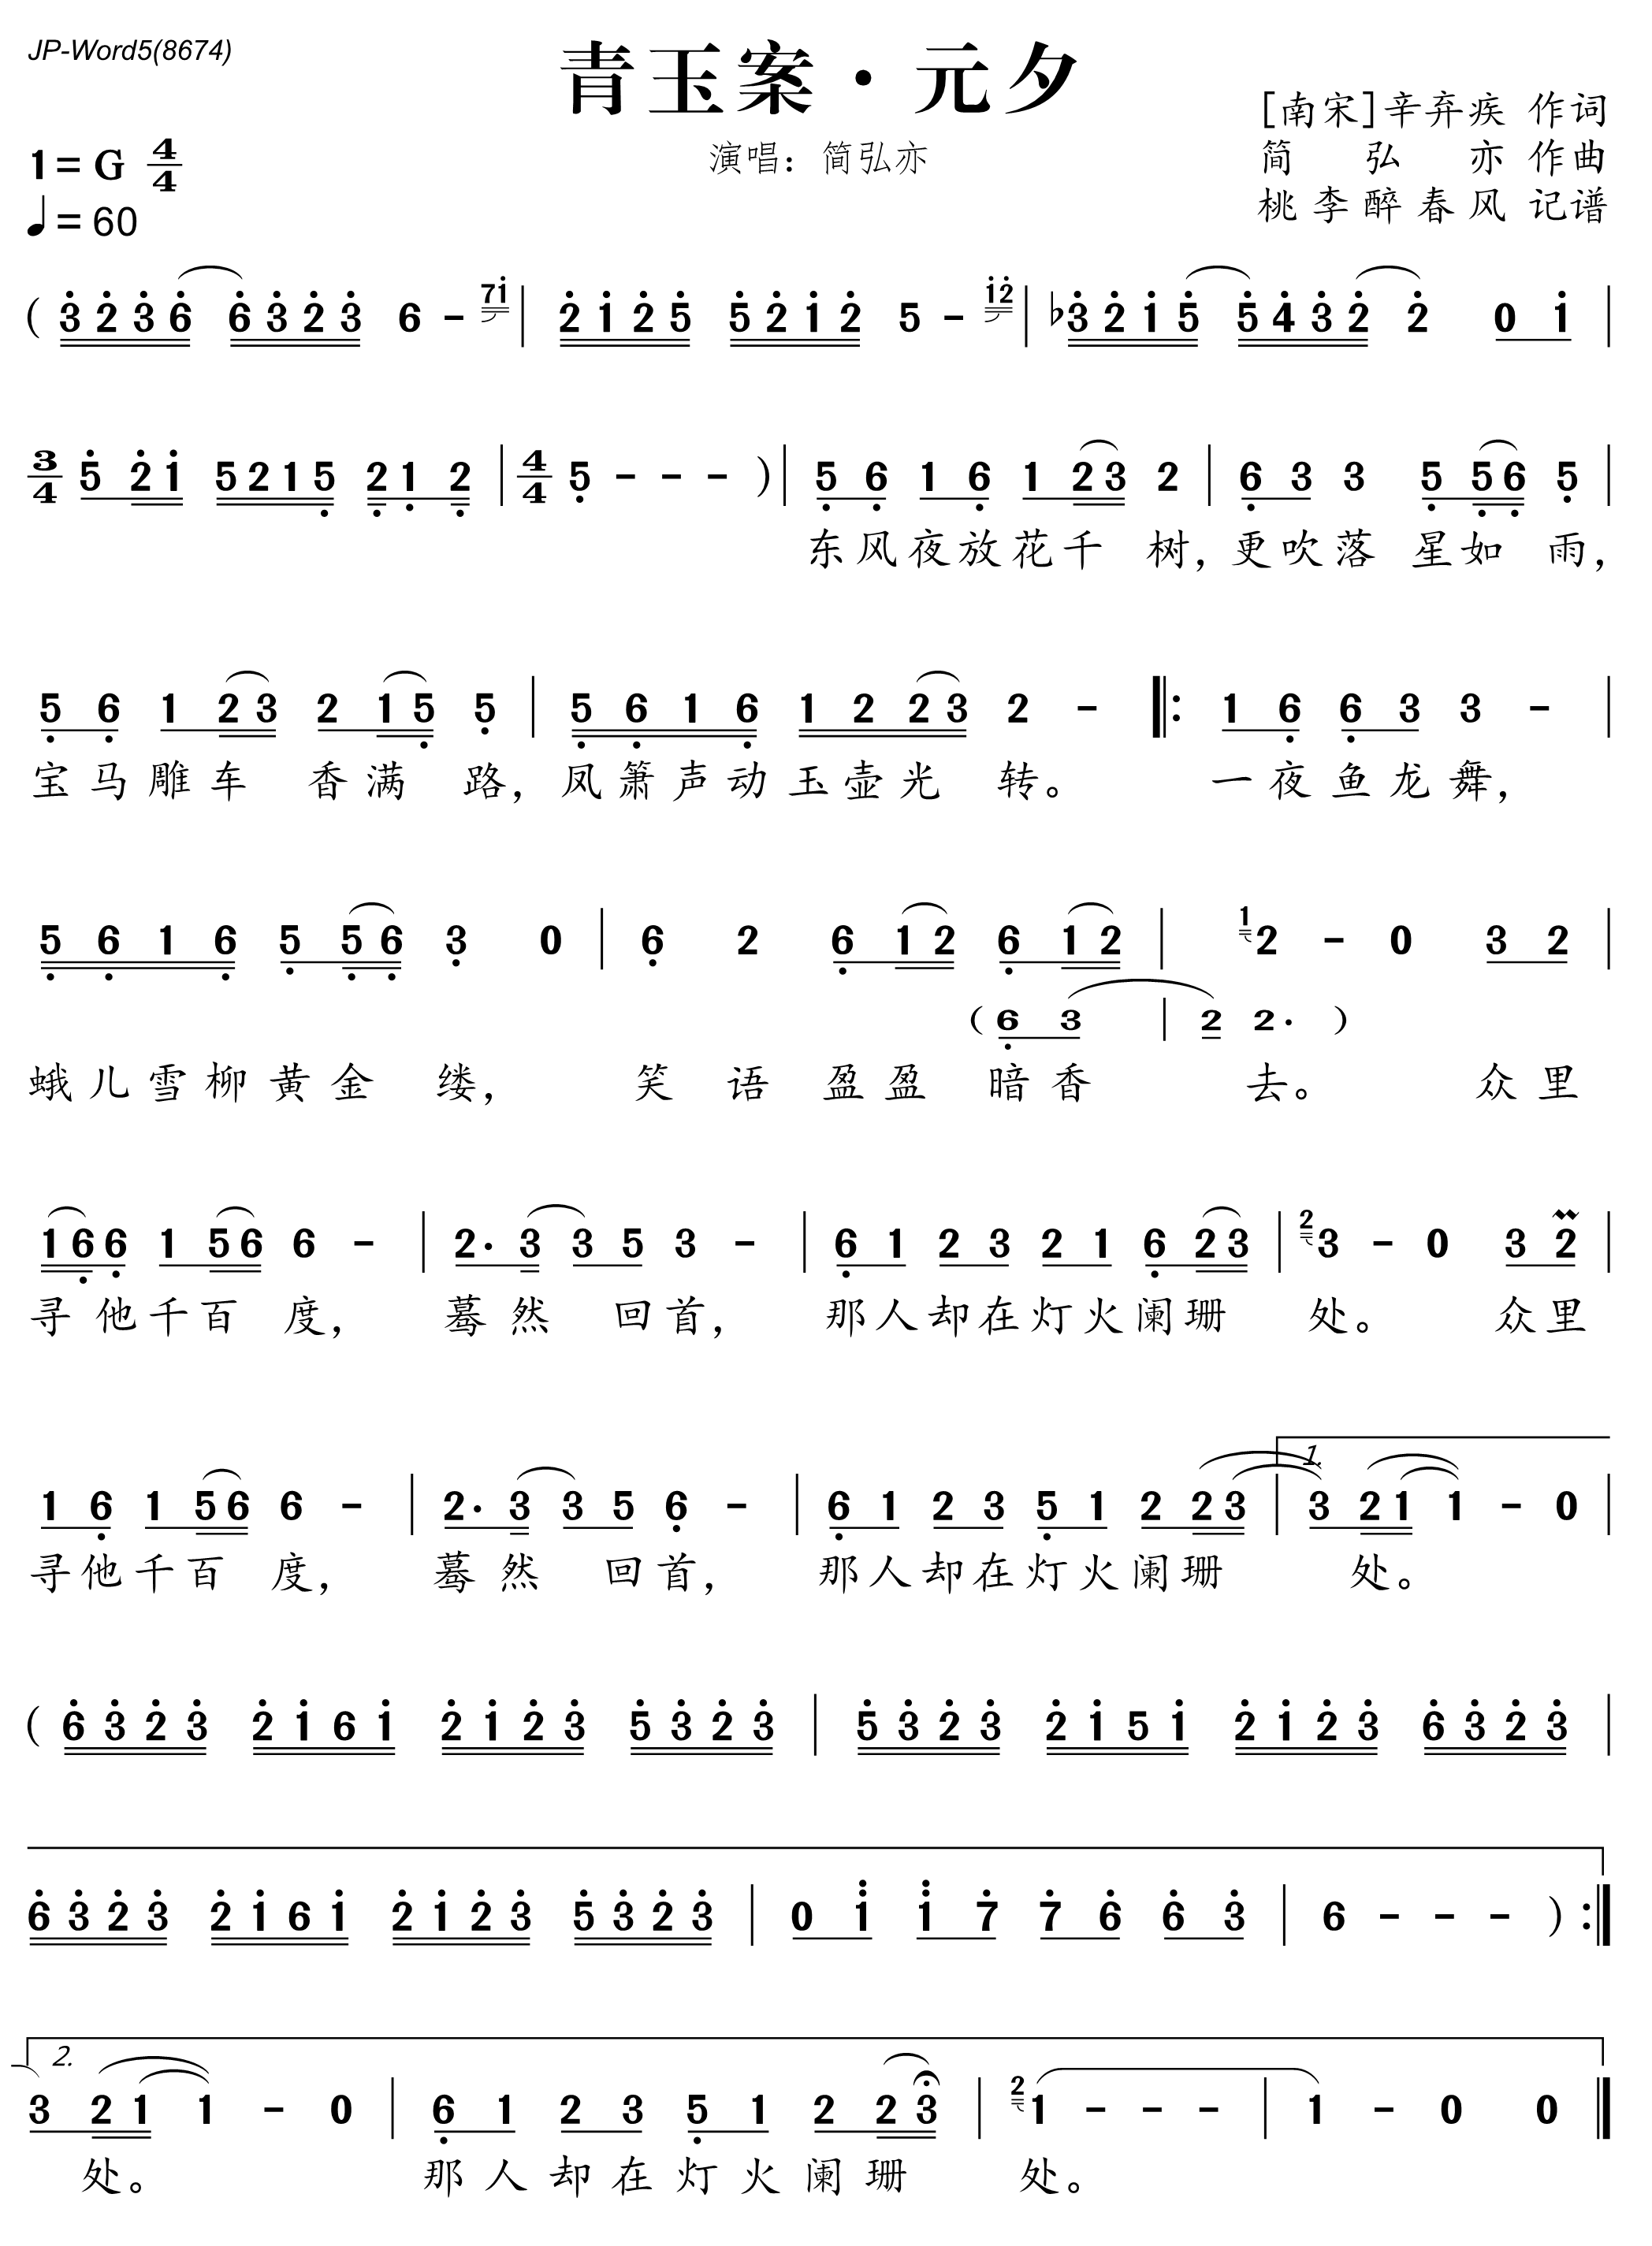
\includegraphics[width=\textwidth]{dongxiao/20200323青玉按.png}
\section{卷珠帘}
    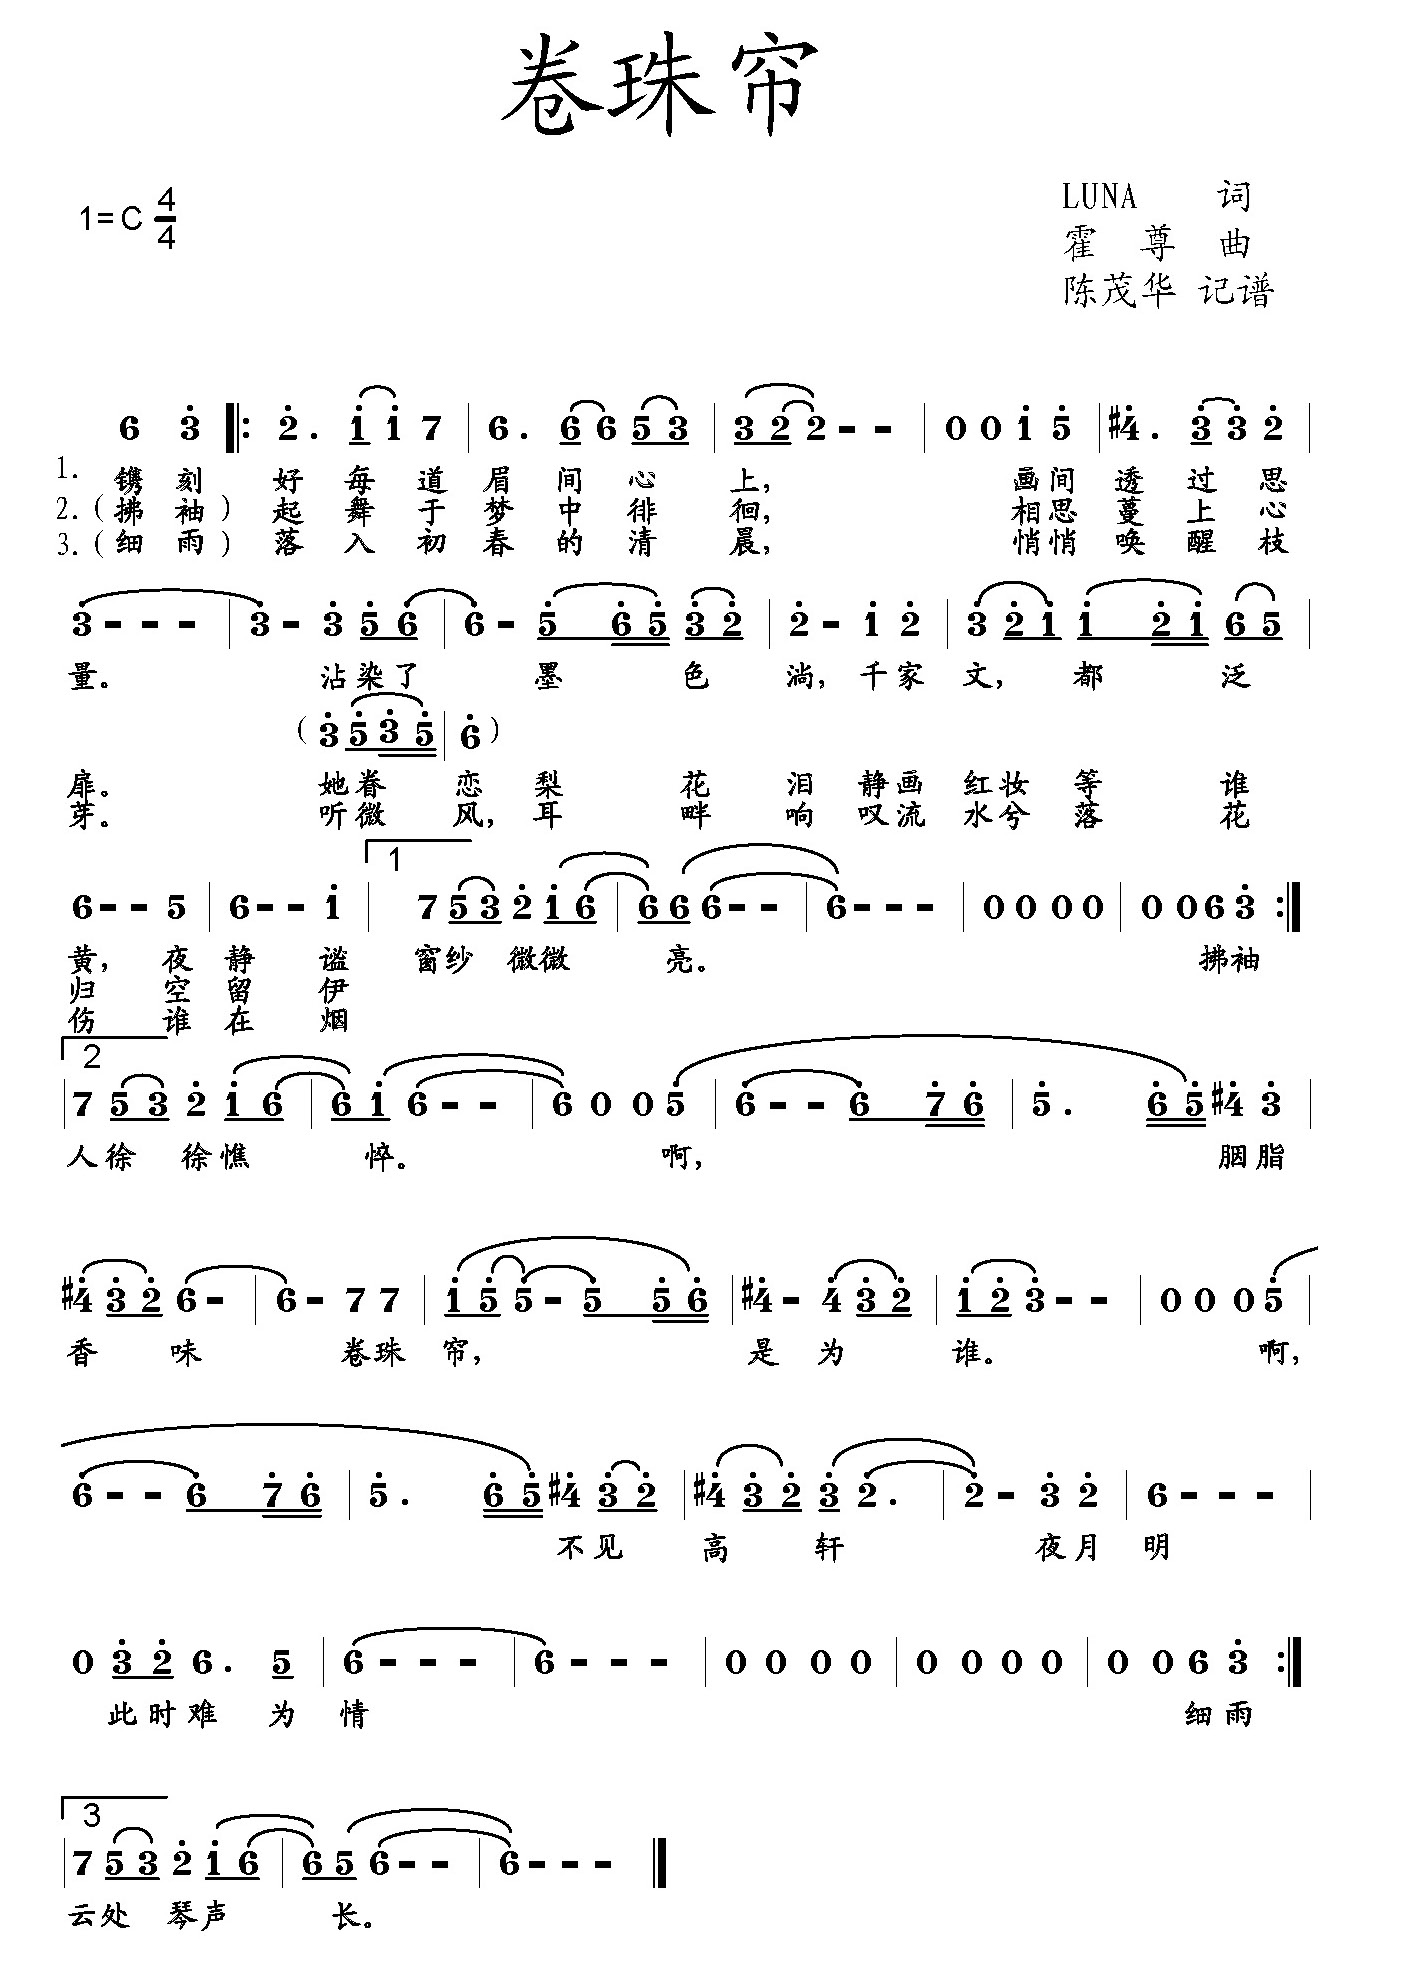
\includegraphics[width=\textwidth]{dongxiao/20200323卷珠帘.jpg}
\section{玉楼春}
    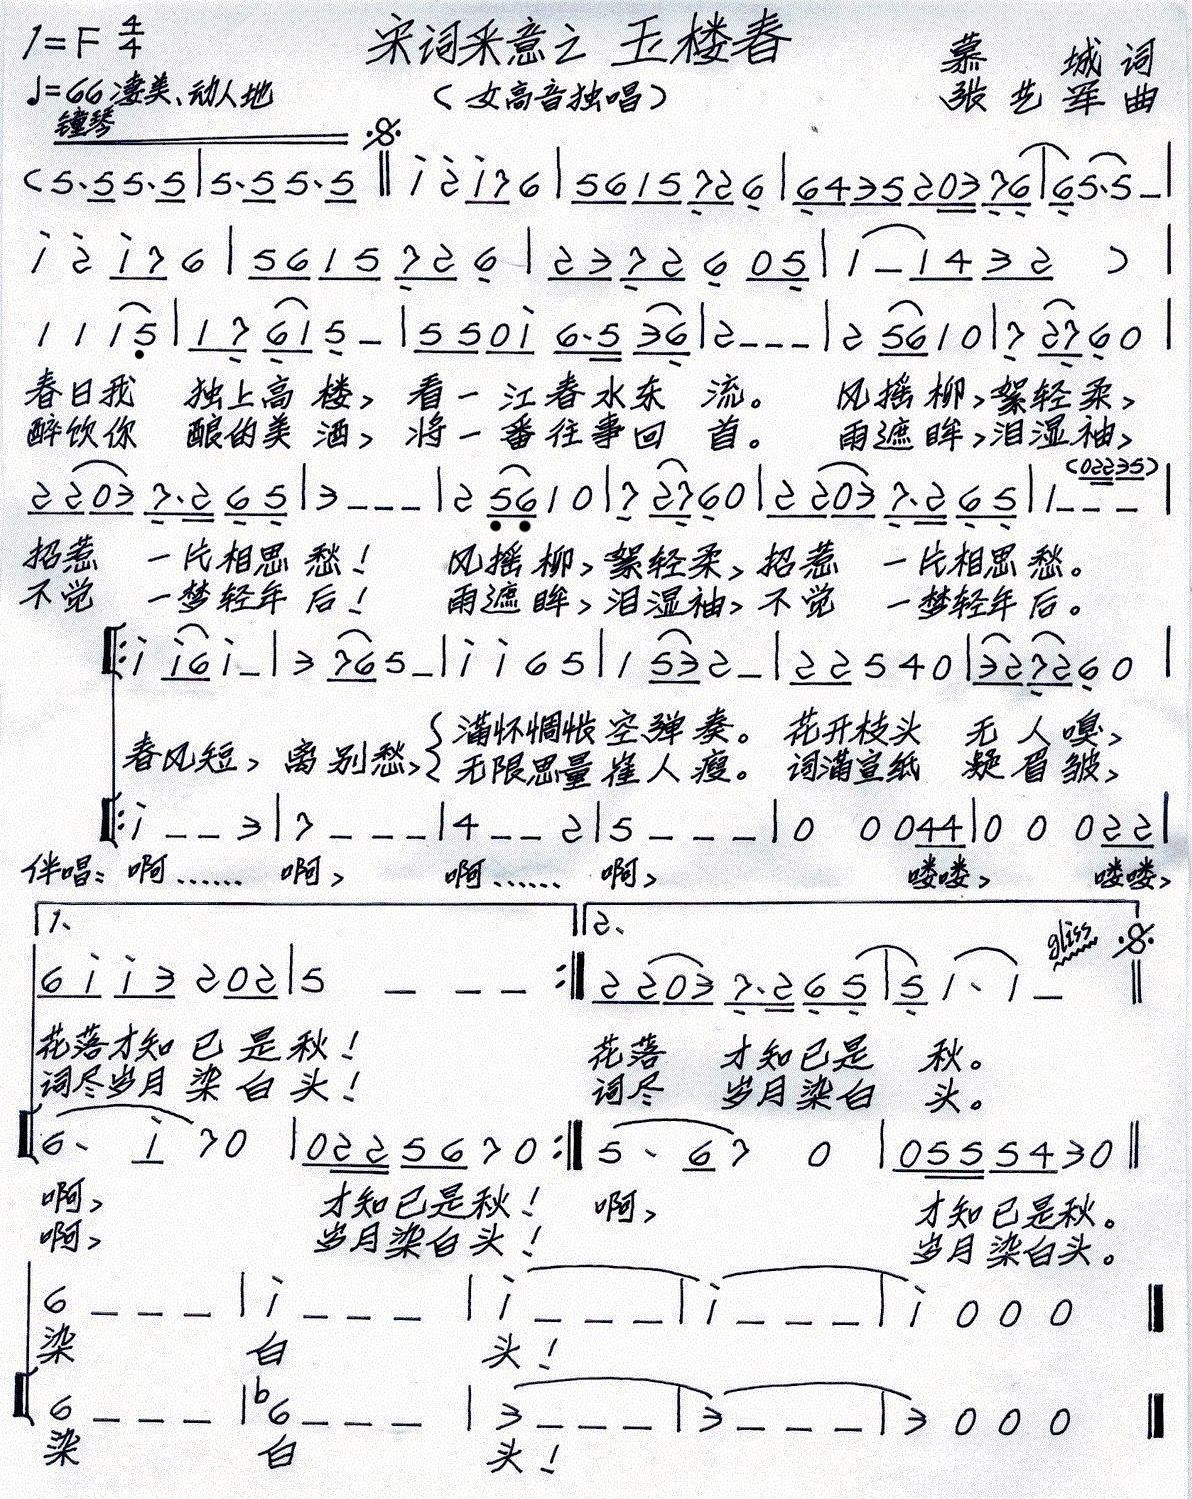
\includegraphics[width=\textwidth]{dongxiao/20200323玉楼春.jpg}
\section{寒香}
    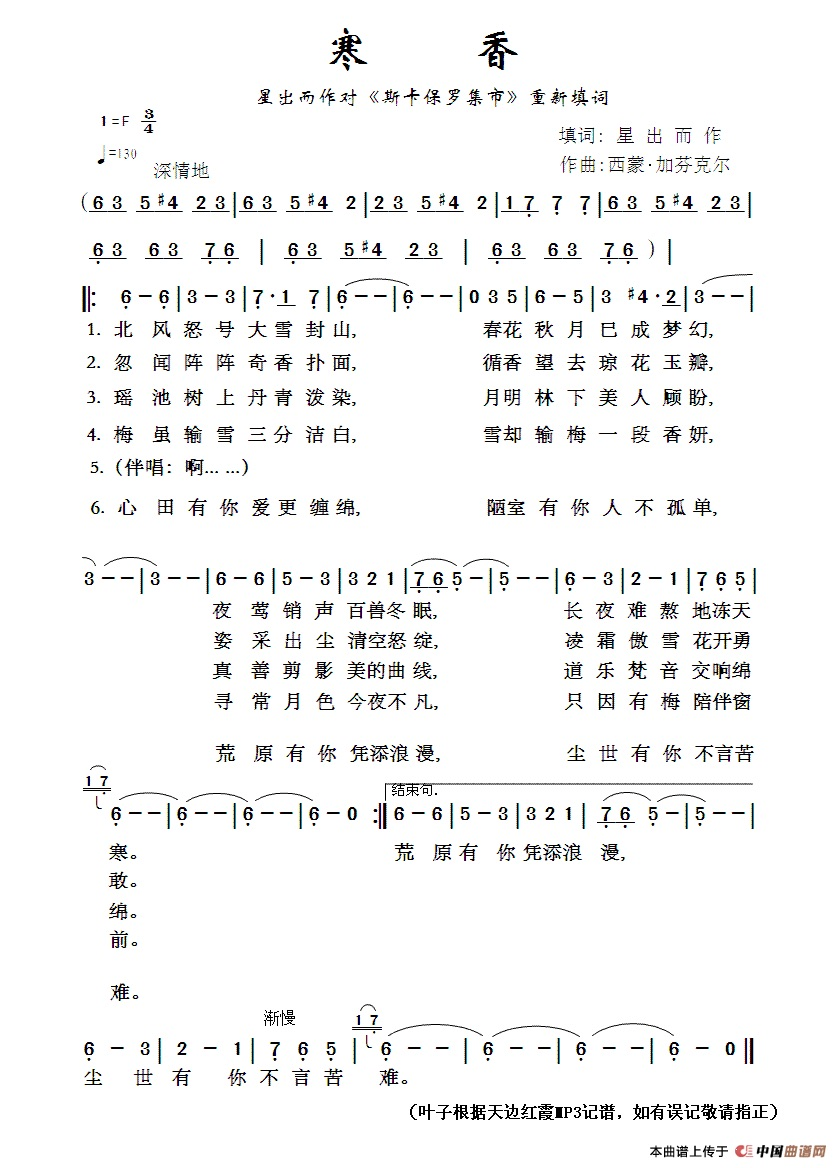
\includegraphics[width=\textwidth]{dongxiao/20200323寒香.jpg}
    
\section{初见}
    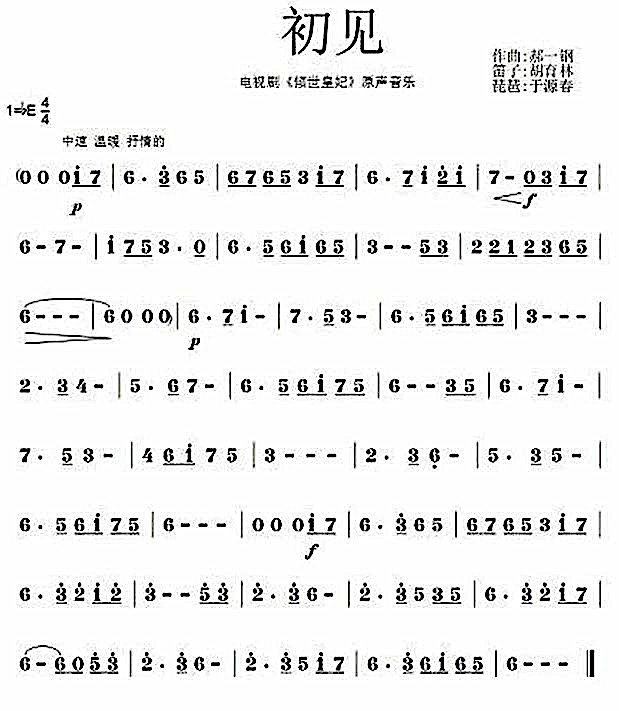
\includegraphics[width=\textwidth]{dongxiao/20200323初见.jpg}
\section{白桦林}
    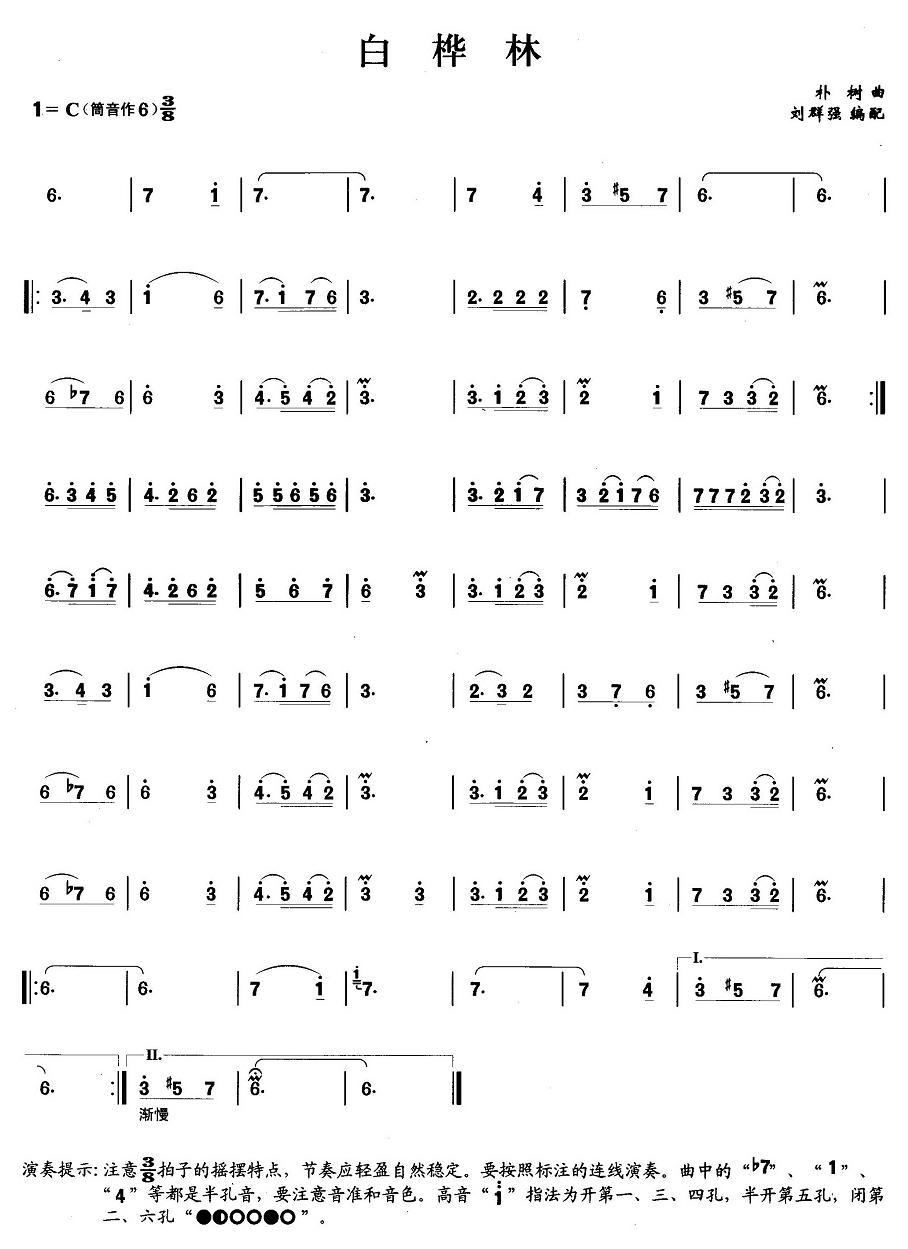
\includegraphics[width=\textwidth]{dongxiao/20200323白桦林.jpg}
\section{揽工调}
    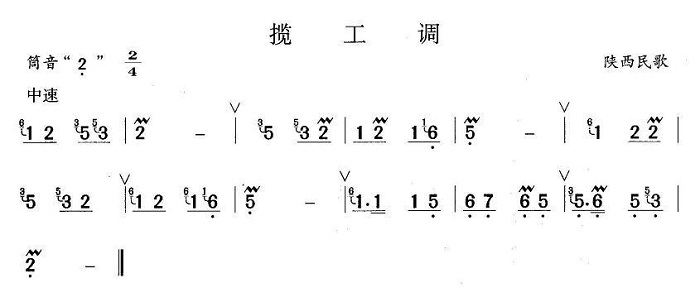
\includegraphics[width=\textwidth]{dongxiao/20200323揽工调.jpg}
    
\section{风留念}
    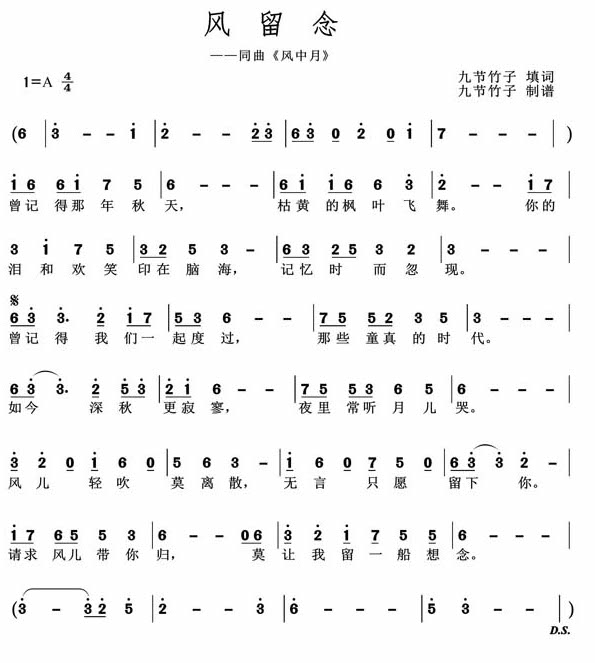
\includegraphics[width=\textwidth]{dongxiao/20200323风留念.jpg}
\section{墨香-长安曲}
    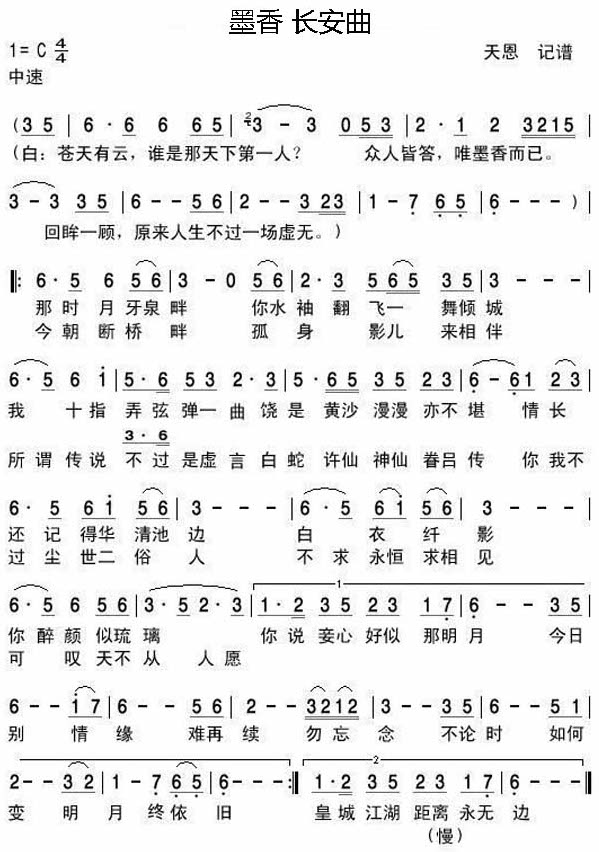
\includegraphics[width=\textwidth]{dongxiao/20200323墨香-长安曲.jpg}

\section{二泉映月}
    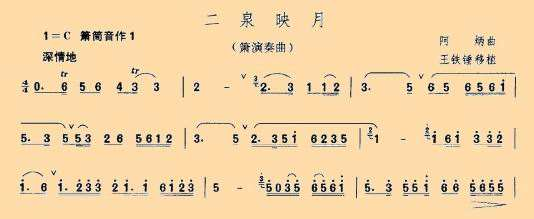
\includegraphics[width=\textwidth]{dongxiao/20200324二泉映月.jpg}  
\section{生离死别}
    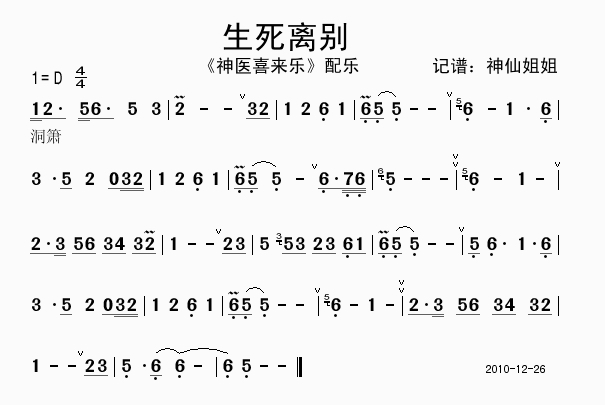
\includegraphics[width=\textwidth]{dongxiao/20200324生离死别.jpg} 
\section{大鱼}
    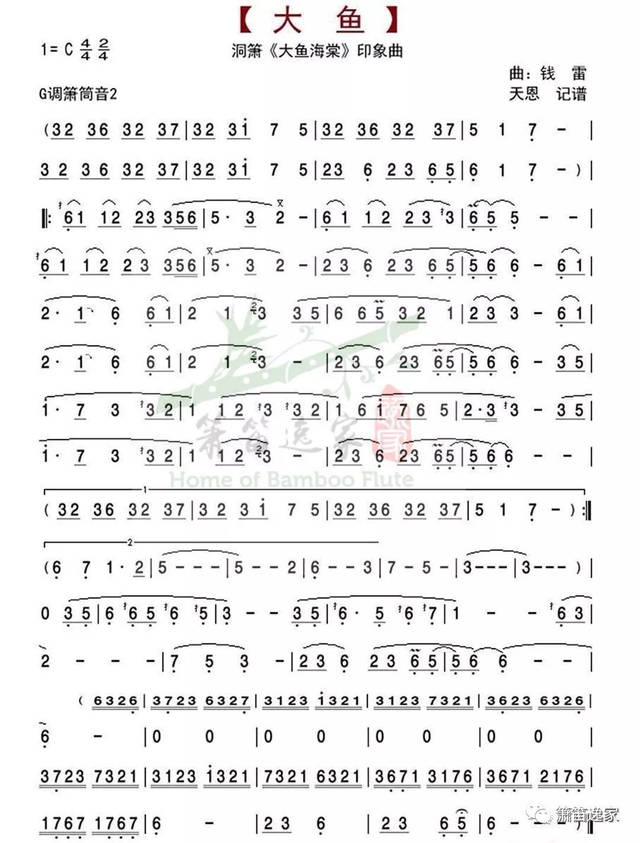
\includegraphics[width=\textwidth]{dongxiao/20200324大鱼.jpg}
\section{天边}
    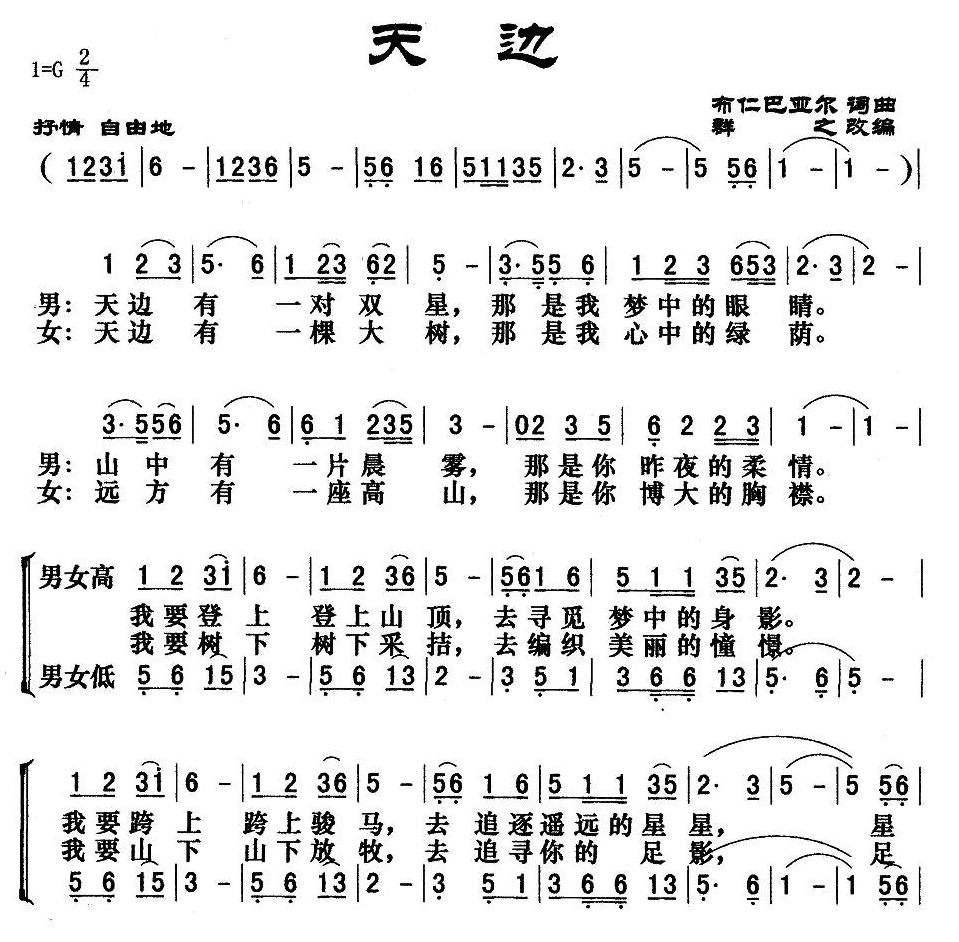
\includegraphics[width=\textwidth]{dongxiao/20200324天边.jpg}


\chapter{技巧练习}
\section{长音练习(1全按作低音5,2全按作低音5)}
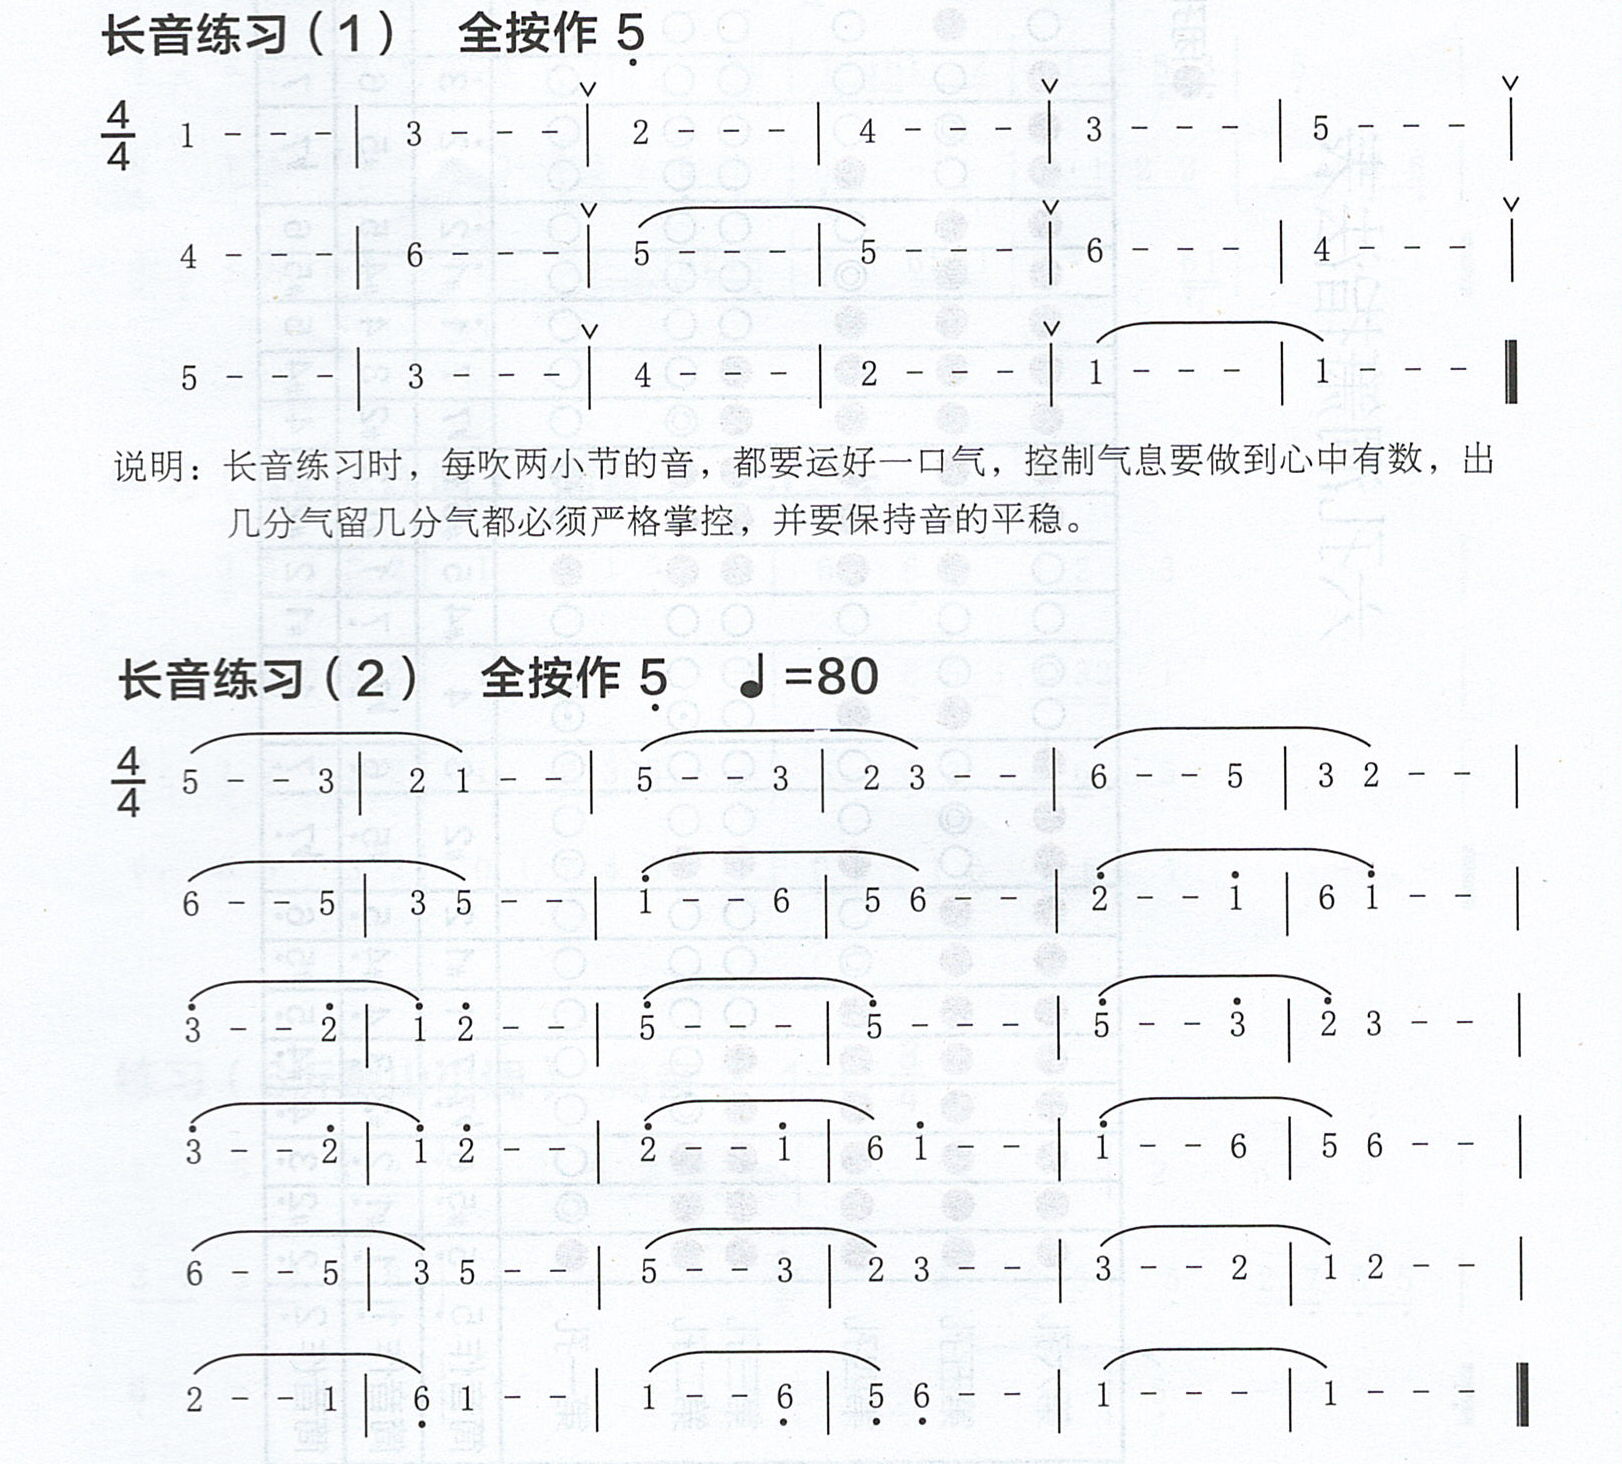
\includegraphics[width=\textwidth]{dongxiao/Scan 7.jpeg}

\chapter{演奏符号}
\section{一}
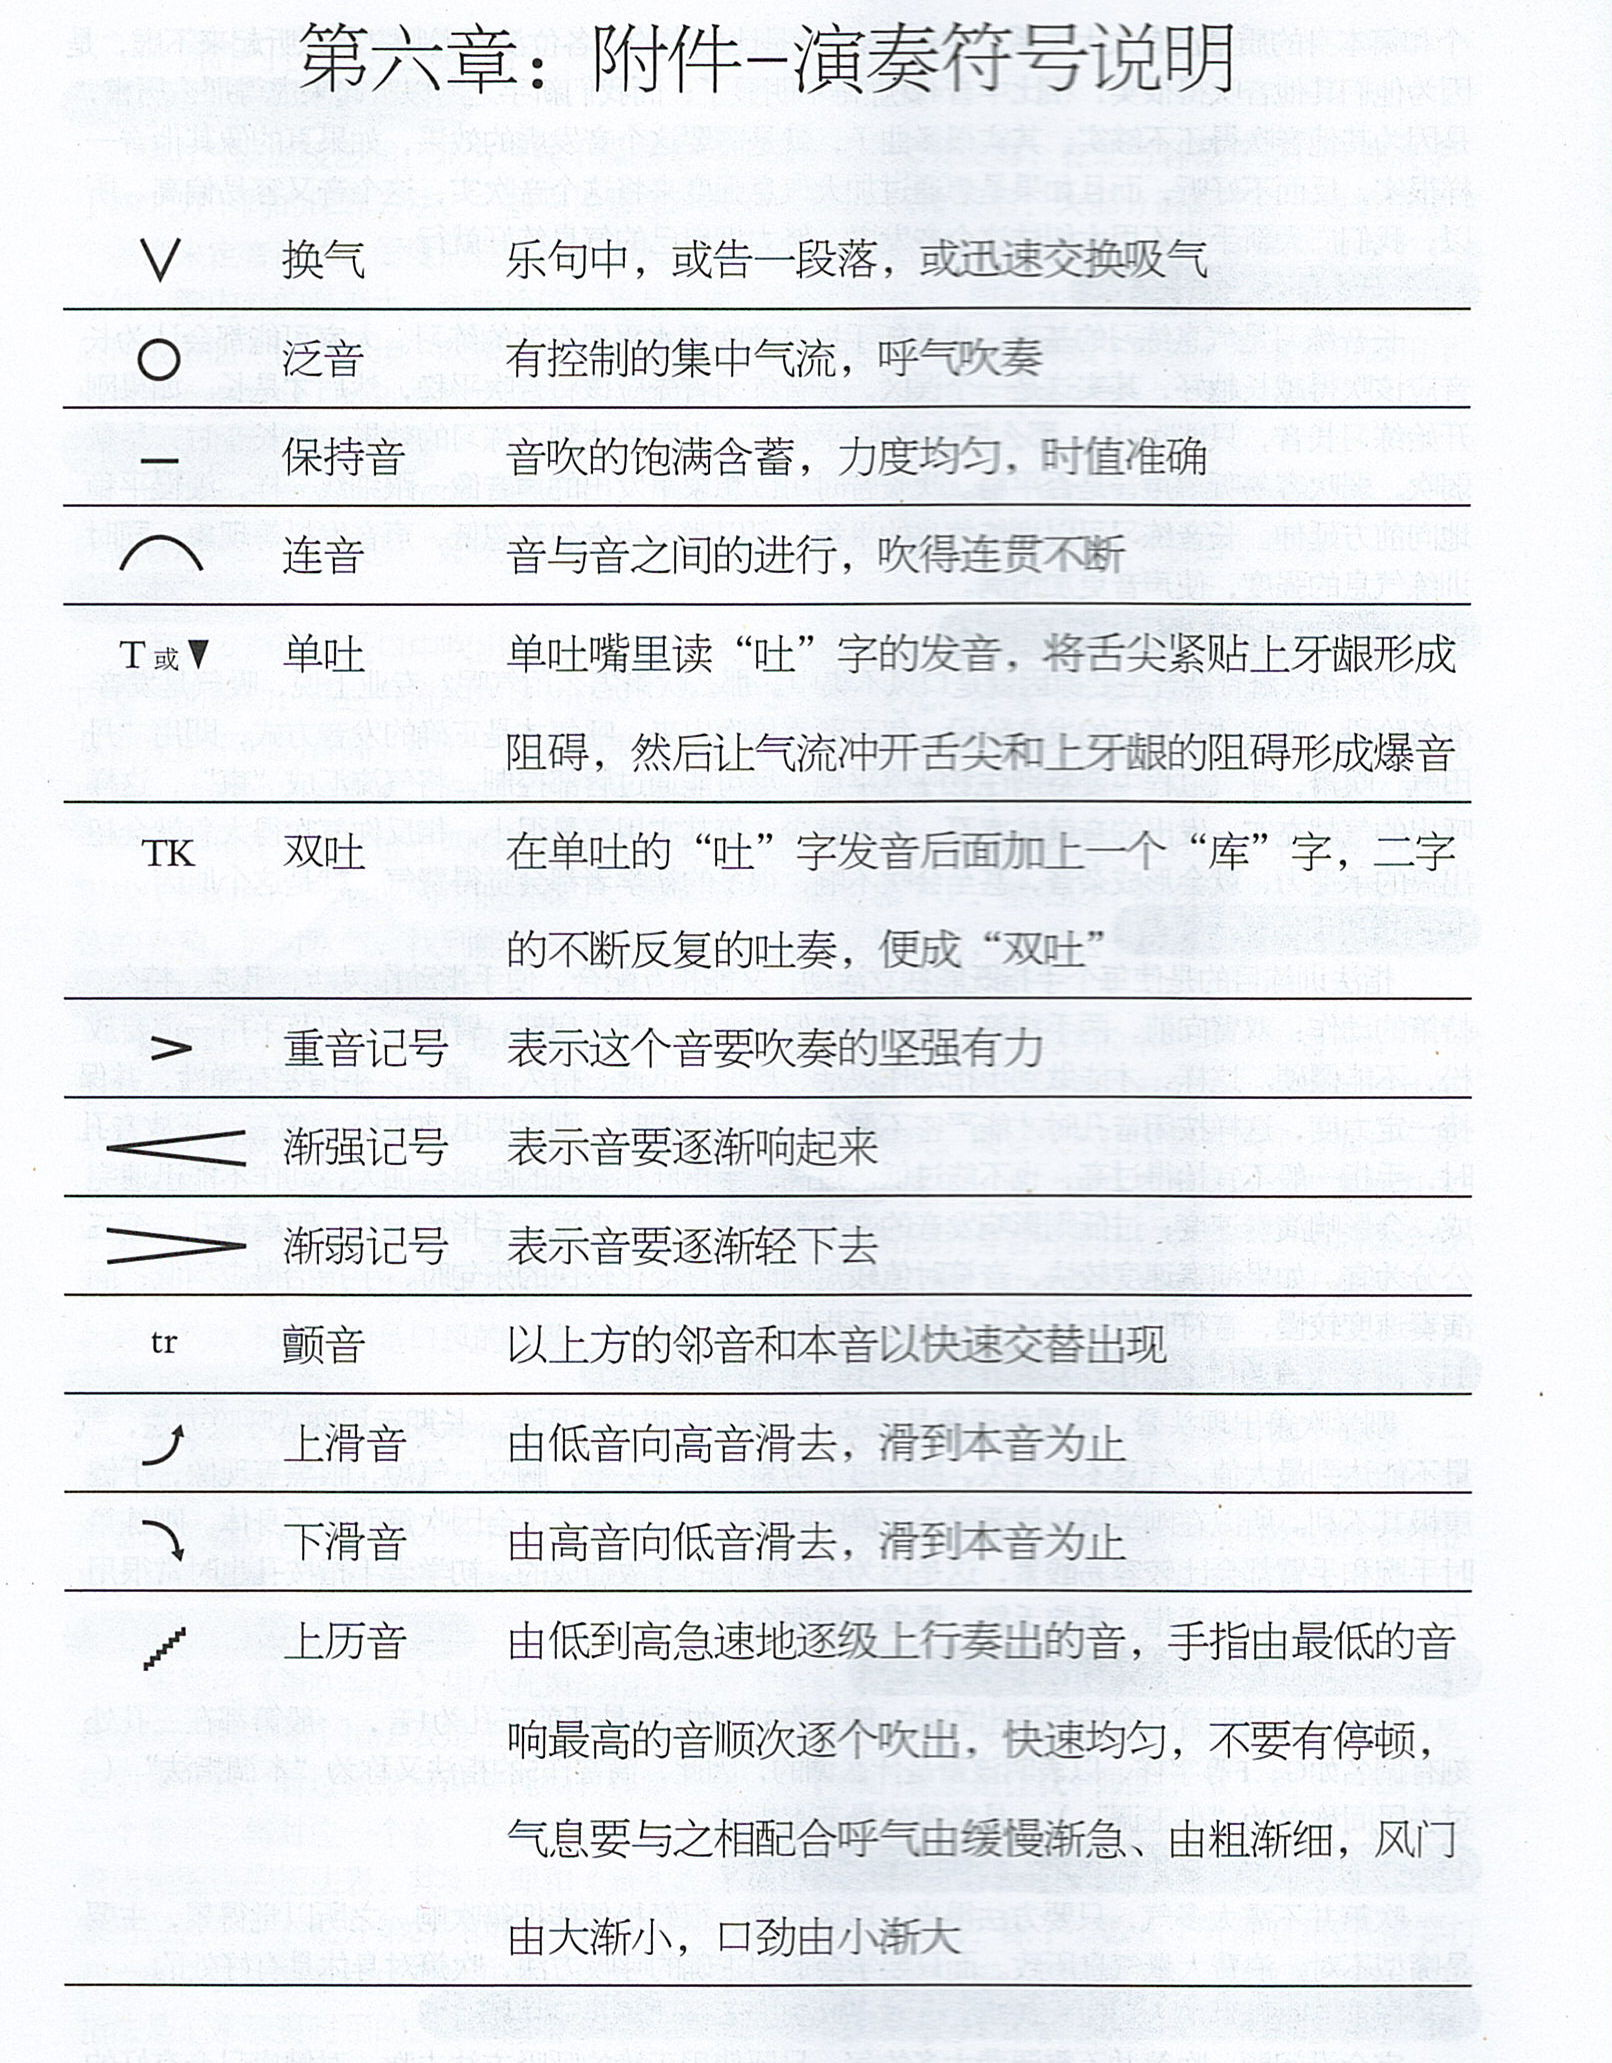
\includegraphics[height=0.8\textheight]{dongxiao/Scan 24.jpeg}
\section{二}
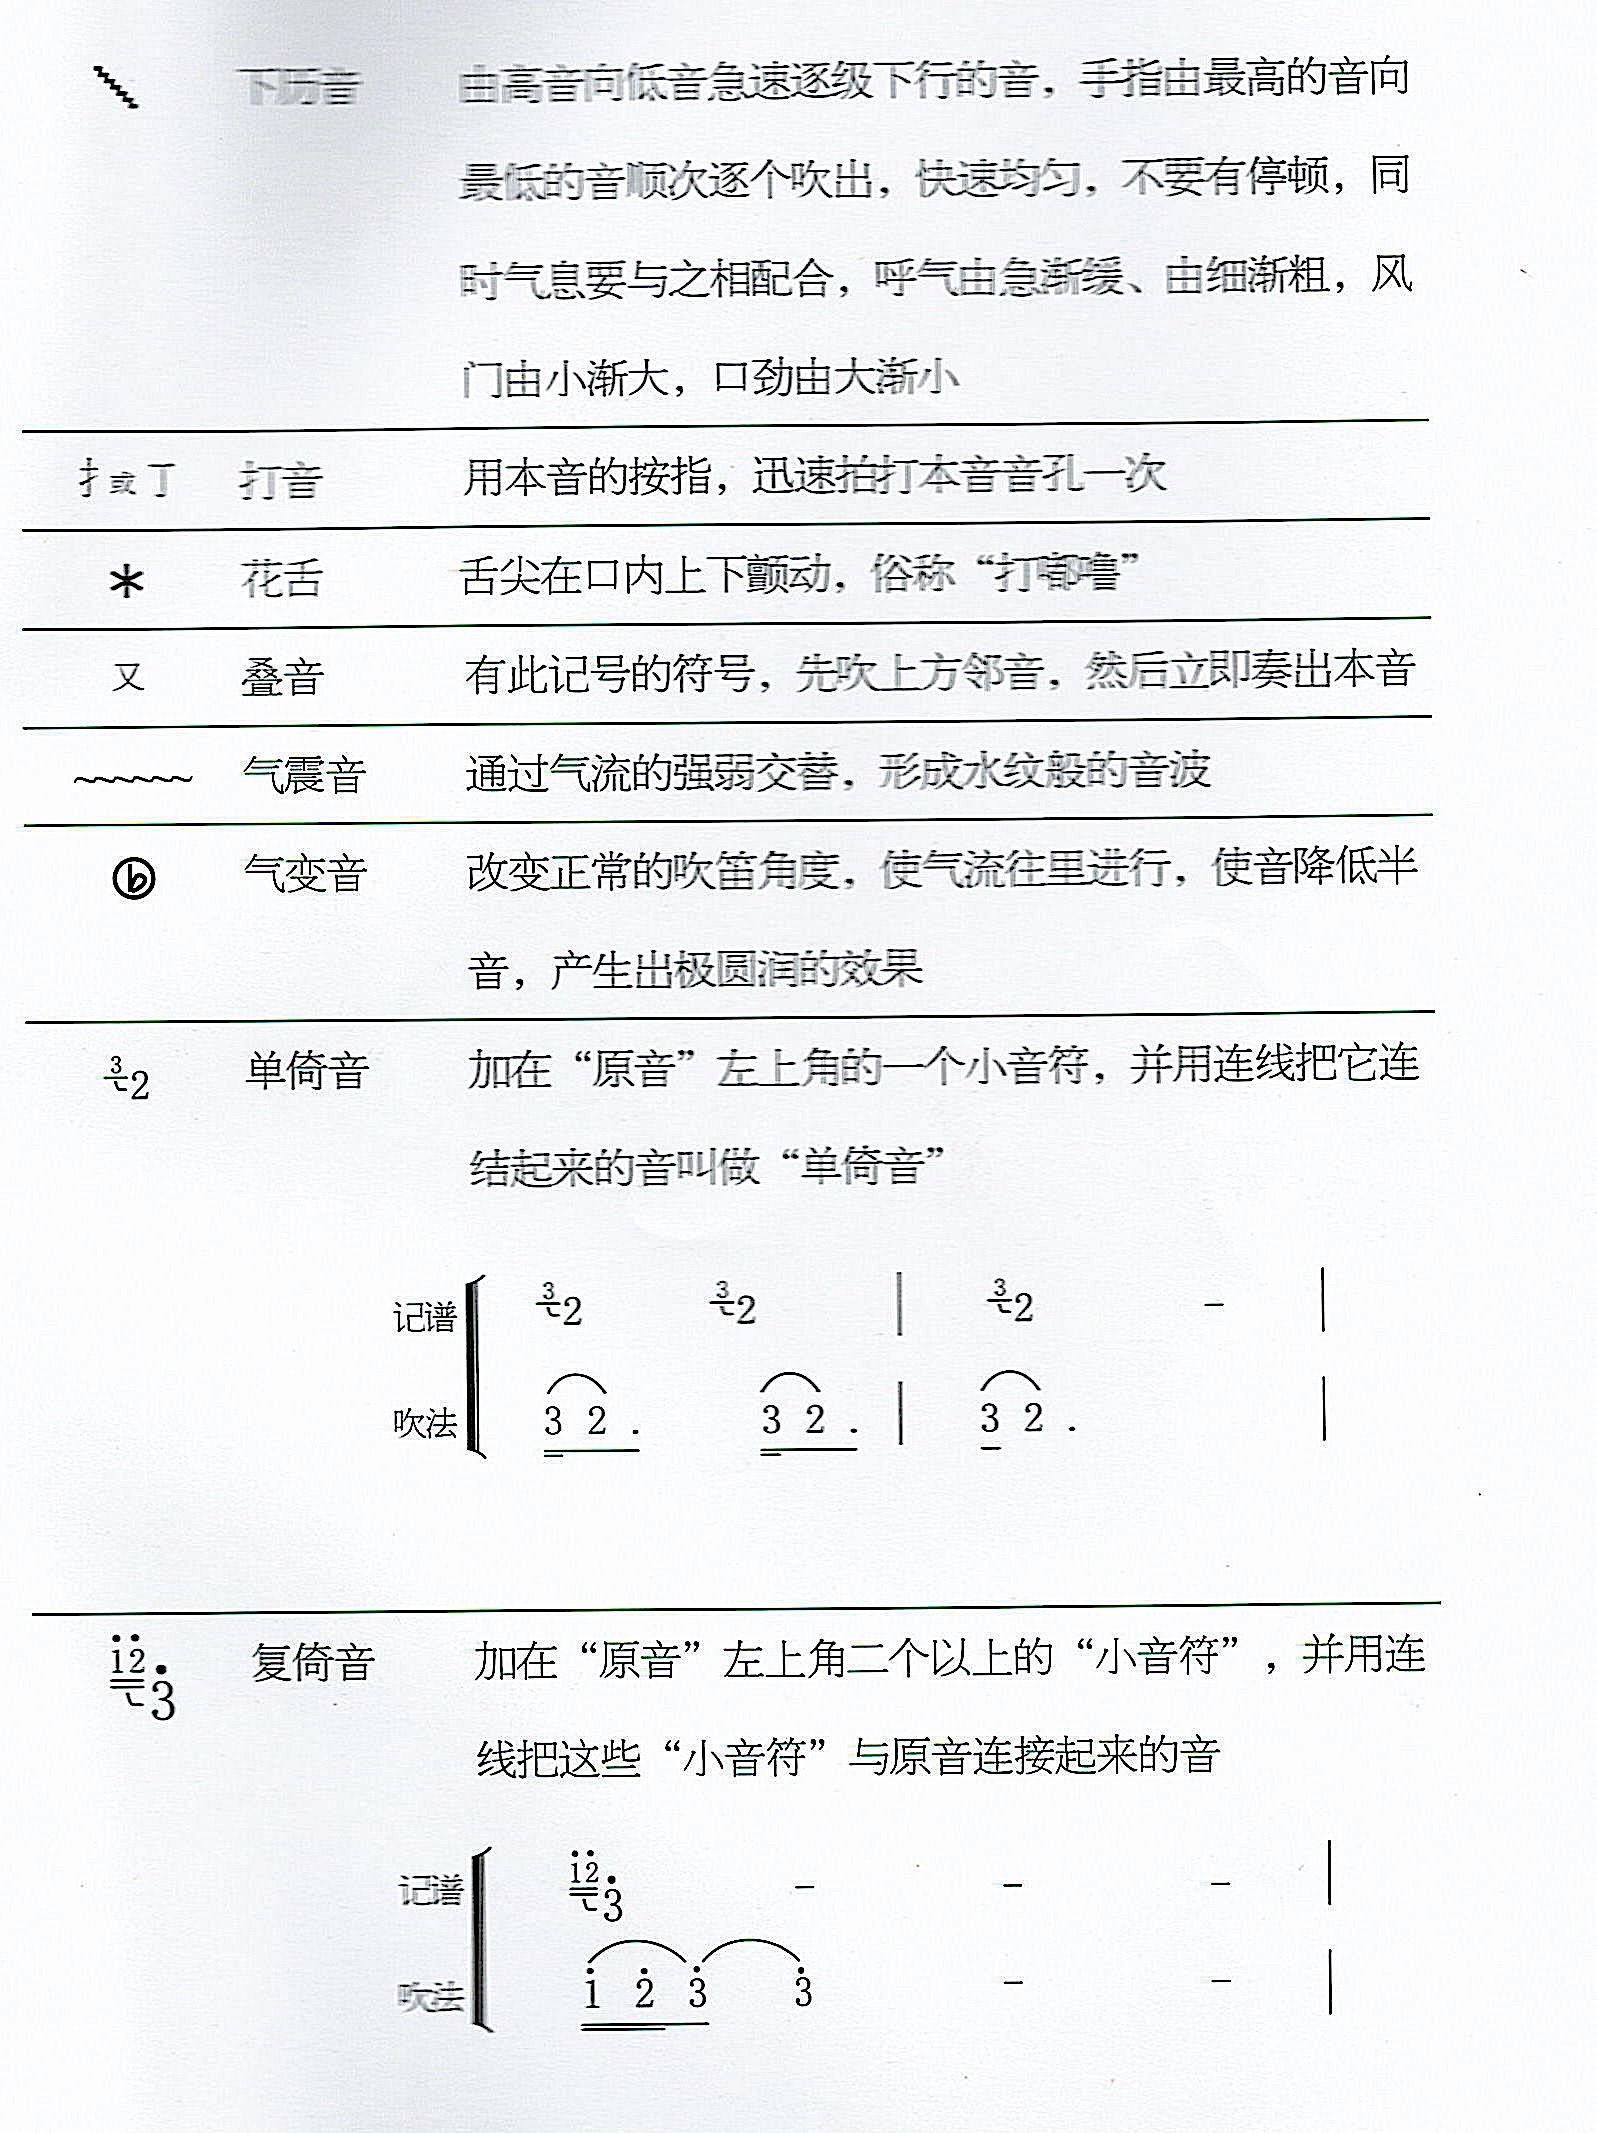
\includegraphics[width=\textwidth]{dongxiao/Scan 25.jpeg}
\end{document}
